%https://medemanabu.net/latex/documentclass/
\documentclass[12pt,oneside]{jbook}
%\documentclass[a4j,12pt,oneside]{jbook}
\usepackage{master_thesis2020}
\usepackage{comment}
\usepackage{amssymb}

\usepackage{booktabs}
\usepackage{siunitx}
\usepackage{breqn}%数式を改行する


%https://www.overleaf.com/learn/latex/Nomenclatures
\usepackage{nomencl}
\makenomenclature
\usepackage{etoolbox}
\renewcommand\nomgroup[1]{%
  \item[\bfseries
  \ifstrequal{#1}{A}{Physics Constants}{%
  \ifstrequal{#1}{B}{Material Properties}{%
  \ifstrequal{#1}{C}{Other Symbols}{}}}%
]}
\newcommand{\nomunit}[1]{%
\renewcommand{\nomentryend}{\hspace*{\fill}#1}}


\begin{document}
\thesistitle
	{Forced convective heat transfer in cylindrical pipe flows} % 論文題目
	{MD18060} % 学籍番号
	{Yoshinori}{Hattori} % 氏名
    {}{}
\tableofcontents

\mbox{}
\nomenclature[A, 02]{$c$}{Speed of light in a vacuum inertial system\nomunit{$299,792,458\, m/s$}}
\nomenclature[A, 03]{$h$}{Plank Constant\nomunit{$6.62607 \times 10^{-34}\, Js$}}
\nomenclature[B, 01]{$T$}{Temperature\nomunit{$K$}}
\nomenclature[B, 02]{$C_{p}$}{Specific heat capasity\nomunit{$J \cdot kg^{-1} K^{-1}$}}
\nomenclature[B, 03]{$\lambda$}{Thermal conductivity\nomunit{$W m^{-1} K^{-1}$}}
\nomenclature[B, 04]{$\mu$}{Dynamic viscosity\nomunit{$Pa \cdot s$}}
\nomenclature[B, 05]{$\rho$}{Density\nomunit{$kg/m^{3}$}}
\nomenclature[B, 06]{$Pr$}{Prandtl number\nomunit{-}}

\nomenclature[C]{$V$}{Constant Volume}
\nomenclature[C]{$\rho$}{Friction Index}
\printnomenclature


\chapter{Introduction}
\section{Study background}
Forced convective heat transfer lies at the heart of many aspect of cooling technology and it is therefore desirable to understand its properties as well as possible.
Effective cooling technology is constantly being required to wide variety of industrial engineering aplication.
To achieve effective coolant system requires comprefensive research of heat transfer coefficient with a wide variety of flow condition.
Although many reserchers have been focusing on experimental and computational research, heat transfer coefficient vary with Reynolds number is still unclear.
To this end, many reserchers have been focusing on heat transfer from experimental and computational research aspect.
However, heat transfer in transitional and turbulent flow is still very challenging task for both experimental and computational research.
\begin{enumerate}
	\item Experimental research\\

	\item Computational research\\
	Direct numerical simuration
	In technology, flows regime and heat transfer plays an important role in considerting engineering issues.
	Navie-Stokes equations describe the relation of variable flows.
	\begin{equation}
		\
	\end{equation}
	However, deterministic solution of the equations are only valid for small disturbances in the initial and boundary condition.
	In physically, it is hard to get initial and boundary conditions in infinite accurate.
	Turbulent has a large amount of fluctuations, i.e. turbulent is completely different kind of laminar flows.
	Direct Numerical Simuration (DNS) is one of the simulation way to predict flow forms.
	The object of the simuration is to solve the compelete set of equation of motion without using any model.
	From Kolmogorov lenght scale, total number of cumputations is derivered following equation (\ref{DNS_total_number_of_computation}).
	The DNS require large amount of total number of computations.
	\begin{equation}
	    \mathcal N \times \mathcal M= \mathcal O (Re^{11/4})
	    \label{DNS_total_number_of_computation}
	\end{equation}
	The equauation implies the limitation of the DNS and that is directly connected to computer technology.
	Normally, engineeres is interested in high Reynolds number such as aircraft or atmospheric boundary layer.
	However, such high Reynolds number requires huge amount of total number of computations and it's far from reality.
	Large eddy simulation
\end{enumerate}

One attempt to improve our understanding of entanglement is the study of our ability to perform experimental investigation


These coolant technology is used wide varaety of coolant applications such as electric devices, automotive, and plant factory.
Considering heat transfer issues, heat transfer coefficients are one of the most important numbers.
The Nusselt number (Nu) is a dimensionless number which represents the ratio of convective (h) and conductive heat transfer (k), as expressed in Equation.
\section{Previous research}

The equauation implies the limitation of the DNS and that is directly connected to computer technology.
Normally, engineeres is interested in high Reynolds number such as aircraft or atmospheric boundary layer.
However, such high Reynolds number requires huge amount of total number of computations and it's far from reality.

Therefore, it is nessesary to get experimental data for correlations of heat transfer and flow condition and the Reynolds number.

%attention!!!!!!!!!!!
Many studies have pointed out that a heat transfer coefficient varies depending on the type of flow: laminar, transition and turbulent.
Gnienlinski\cite{Gnielinski1975}\cite{Gnielinski1976} showed a calculation method about heat transfer coefficients for the laminar, transitional and turbulent flows.
Bertsche et al.\cite{Bertsche2016} focused on reliable prediction of the heat transfer coefficient for transitional flows.
In their study, they showed experimental the heat transfer coefficients for the Reynolds number, $500 < Re < 23000$, and the Prandtl number, $7 < Pr < 41$.\\
However, not so many data is available for experimental data of laminar-to-turbulent transitional region.
More studies should be conducted to obtain experimental data for high the Prandtl number and transitional flows.
In this study, the author focused on forced convective heat transfer in flow of water and glycole in a cylindrical pipe.
A 50/50vol\% mixture of water and glycole, which is a typical liquid coolant in automotive applications, was used as an operating fluid.
The experiment was carried out by considering a board range of Reynolds numbers, spanning from a laminar to fully turbulent flow.
Moreover, the measurements of the wall friction coefficients was also performed in this study.


\subsection{Skin friction coefficients}
The skin friction coefficients for laminar flow is descrived following equation.
\begin{equation}
    C_{f,lam}=\frac{16}{Re_{b}}
    \label{cf_laminar}
\end{equation}

Konakov\cite{Petukhov1970} showed the skin friction coefficients for turbulent flow.
\begin{equation}
	C_{f,turb}=0.25(1.8log(Re_{b})-1.64)^{-2}
	\label{cf_turbulent}
\end{equation}

\subsection{The heat transfer coefficients}
Gunienski \cite{Gnielinski2013} showed correlations for each flow conditions: laminar, transitional and turbulent, respectively.
Gunienski \cite{Gnielinski2013} showed calculation method for laminar flow.
\begin{equation}
    Nu_{lam}=(3.66^{3}+0.7^{3}+(1.615(Re_{b}Pr_{b}\frac{d_{i}}{L})^{1/3})^{3})^{1/3}
    \label{Nu_laminar}
\end{equation}
%The range 0.1<<Pr_{b}<<1000, 10^{4}<<Re_{b}<<10^{6}.
He showed calculation method for turbulent flow.
\begin{equation}
    Nu_{turb}=\frac{\frac{C_{f,turb}}{2Re\cdot Pr_{b}}}{1+12.7 \sqrt{\frac{C_{f,turb}}{2}}(Pr_{b}^{2/3}-1)}\cdot (\frac{Pr_{b}}{Pr_{w}})^{0.11}
    \label{Nu_turbulent}
%Nu_{turb}=\frac{\frac{C_{f}}{2\cdot Re\cdot Pr_{b}}{(1+12.7\frac{C_{f}}{2}}\cdot (Pr^{\frac{2}{3}}-1)}\cdot(1+(\frac{d_{h}}{l})^{\frac{2}{3}})\label{Nu_turblent}
\end{equation}
The range is
\begin{equation}
    0.1<<Pr_{b}<<1000, 10^{4}<<Re_{b}<<10^{6}
\end{equation}
He presented transitional flow as a liner interpolation between turbulent and laminar flow.
\begin{equation}
    Nu_{m}=(1-r)Nu_{m,lam}+rNu_{m,turb}
    \label{Nu_transitional}
\end{equation}
\begin{equation}
    r=\frac{Re_{b}-2300}{10^{4}-2300}
	\label{Nu_transitional2}
\end{equation}

\chapter{Methodology}
\section{Material properties}

\subsection{Parameters}
A 50/50vol\% mixture of water and glycole which is a typical liquid coolant in automotive applications were used as a operating fluid.
The material properties of the operationg fluid is temperature dependecy.
As bigger temperature difference between a pipe wall and the bulk, the material properties pronounced.


specific heat capacity
\begin{equation}
	c_{p} = A_{c_{p}}+B_{c_{p}} T = 2.0148 + 4.50E-3T
	\label{Cp}
\end{equation}
\begin{figure}[ht]
	\vspace{0zh}
	\begin{center}
		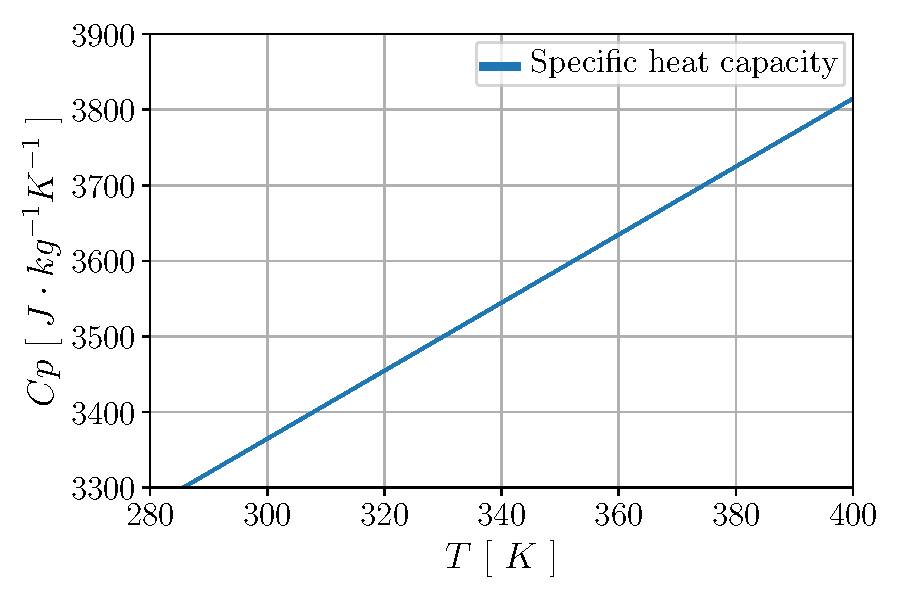
\includegraphics[width=0.65\linewidth]{fig/mp_cp.pdf}
		\vspace{-1zh}
		\caption{Specific heat capacisty vary with temperature}
		\label{cp}
	\end{center}
	\vspace{0zh}
\end{figure}


thermal condictivity
\begin{equation}
	\lambda = A_{\lambda}+B_{\lambda} T = 0.2134 + 6.071E-4T
	\label{lambda}
\end{equation}
\begin{figure}[ht]
	\vspace{0zh}
	\begin{center}
		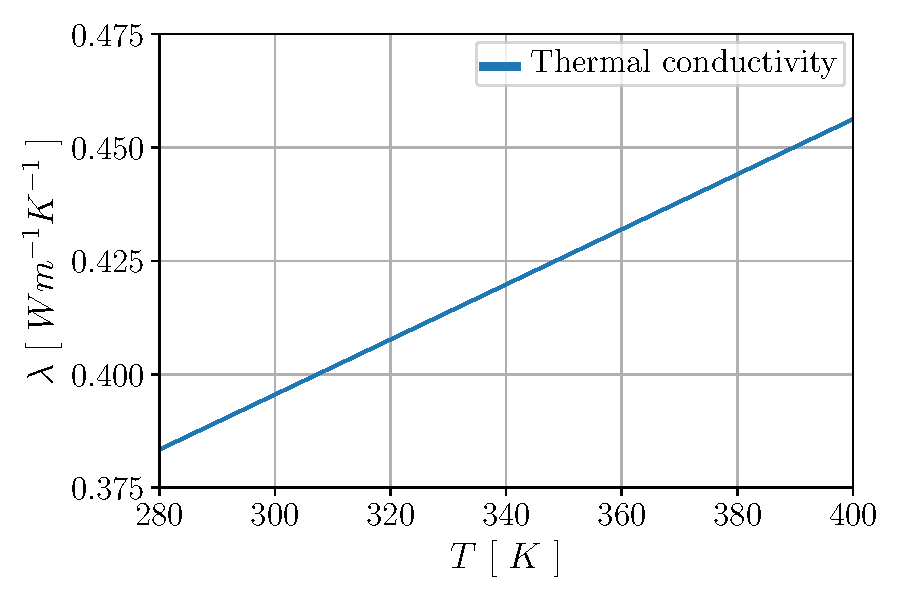
\includegraphics[width=0.65\linewidth]{fig/mp_lambda.pdf}
		\vspace{-1zh}
		\caption{Thermal conductivity vary with temperature}
		\label{lambda}
	\end{center}
	\vspace{0zh}
\end{figure}


dynamic viscosity
\begin{equation}
	\mu = A_{\mu}\cdot \exp \left( \frac{B_{\mu}}{T+C_{\mu}} \right) = 1.1001E-4\exp \left( \frac{325.85}{T-207.30} \right)
	\label{mu}
\end{equation}
\begin{figure}[ht]
	\vspace{0zh}
	\begin{center}
		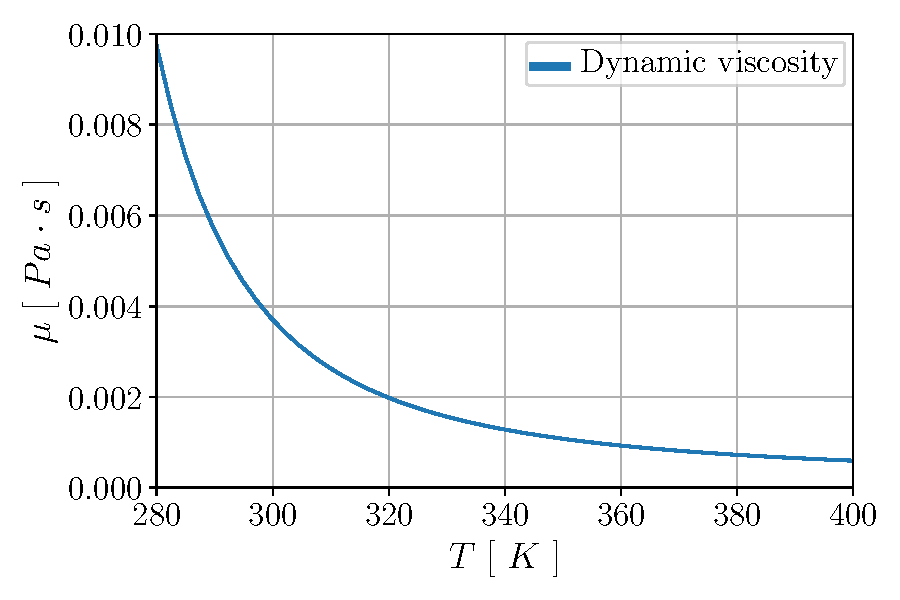
\includegraphics[width=0.65\linewidth]{fig/mp_mu.pdf}
		\vspace{-1zh}
		\caption{Dynamic viscosity vary with temperature}
		\label{mu}
	\end{center}
	\vspace{0zh}
\end{figure}


density
\begin{equation}
	\rho = A_{\rho}+B_{\rho} T = 1268.28 -0.66T
	\label{rho}
\end{equation}
\begin{figure}[ht]
    \vspace{0zh}
	\begin{center}
		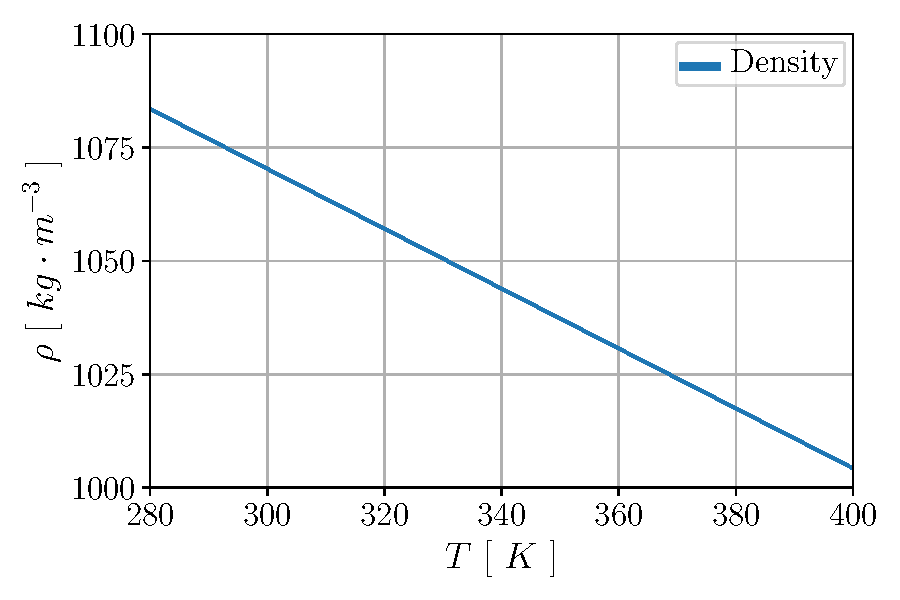
\includegraphics[width=0.65\linewidth]{fig/mp_rho.pdf}
		\vspace{-1zh}
		\caption{Density vary with temperature}
		\label{rho}
	\end{center}
	\vspace{0zh}
\end{figure}


prandtl number
\begin{equation}
	Pr = \frac{\nu}{\alpha}= \frac{\mu \cdot c_{p}}{\lambda}
	\label{pr}
\end{equation}
\begin{figure}[ht]
	\vspace{0zh}
	\begin{center}
		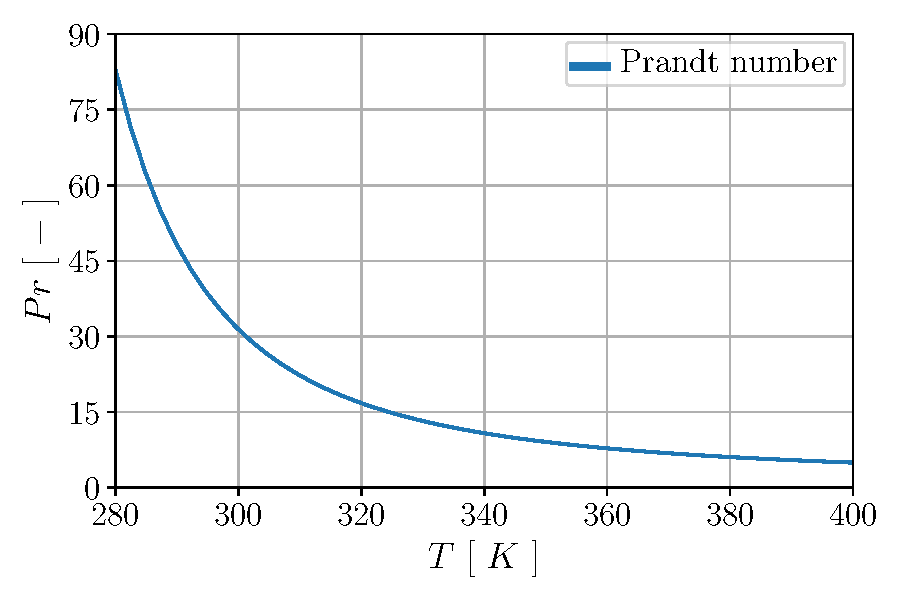
\includegraphics[width=0.65\linewidth]{fig/mp_pr.pdf}
		\vspace{-1zh}
		\caption{Prandtl number vary with temperature}
		\label{pr}
	\end{center}
	\vspace{0zh}
\end{figure}

\subsection{Effect of viscosity and density}
DNS
Effect of viscosity 20\%
Effect og density   0.5\%
experimental

\clearpage

\subsection{Cooling and heating}
Bertsche et al.\cite{Bertsche2016} shows experimental investigation on heat transfer in cylindrical pipe flow by using a 50/50vol\% mixture of water and glycole with cooling.
The operationg fluid is the same as our study, however they measured the heat transfer by cooling the liquid.
For cooling the liquid, the temperature at the wall is lower than bulk temperature.
In other way, for heating the liquid, the temperature at the wall is higher that bulk temperature.
As shown in material properties, the viscosity show strong temperature dependence and the curve isn't linear function.
Thus, the heat transfer doesn't shows the same value with cooling and heating even though a Prandtl number is the same.
\begin{figure}[ht]
    \vspace{0zh}
	\begin{center}
		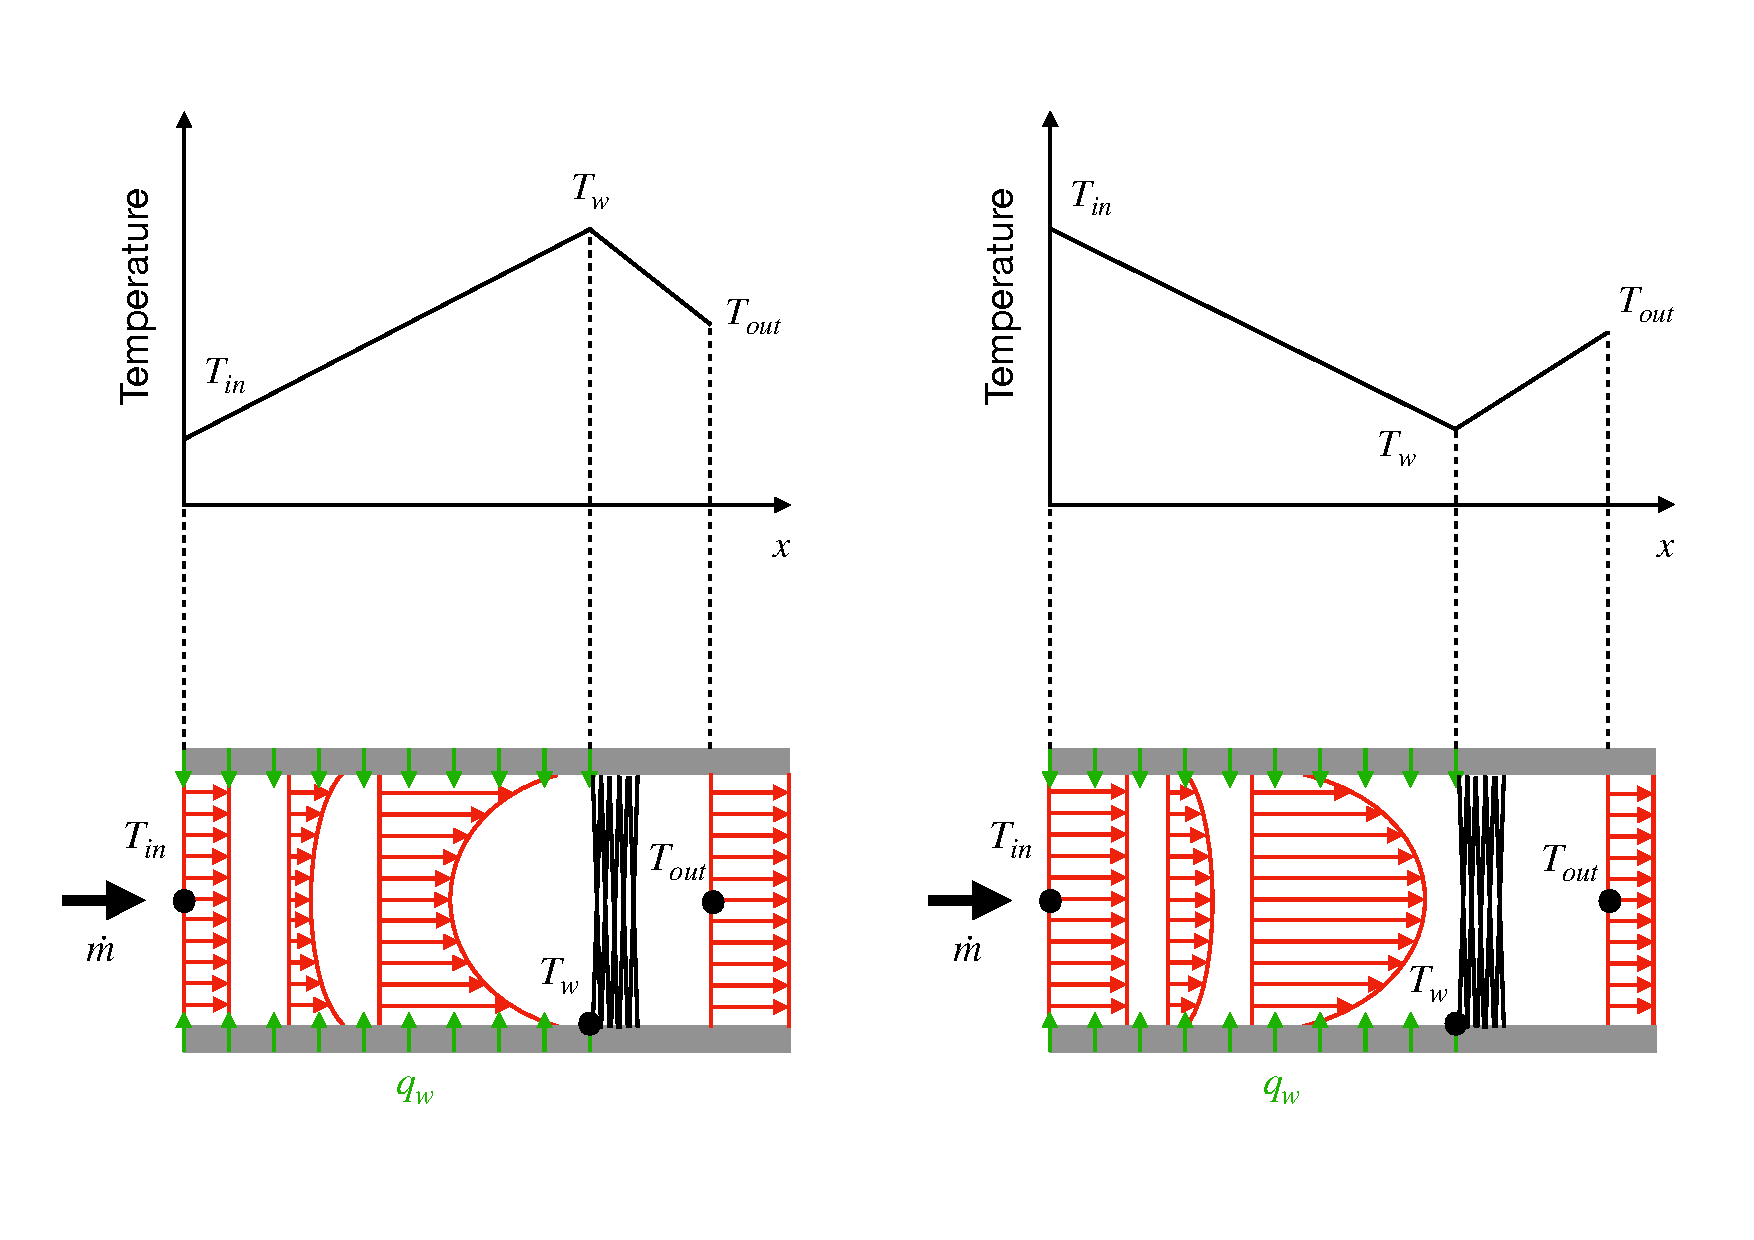
\includegraphics[width=1\linewidth]{fig/heating_and_cooling.pdf}
		\vspace{-2zh}
		\caption{Thermal boundary layer grows in horizontal axis for heating liquid(left) and cooling liquid(right).}
		\label{heating}
	\end{center}
	\vspace{0zh}
\end{figure}

\clearpage
\section{Hydro and thermal boundary layer}

\chapter{Experimental facilities}
\section{Experimental loop}
%Experimental Setup
Figure. \ref{loop} shows a diagram of the experimental loop.
The experimental basically loop consists of a heat exchanger, a pump, a Coriolis mass flow rate, a welder, a reservoir, and a test section.
The heat exchanger keeps a thermal stationary condition in the flow pipe.
The Coriolis mass flow rate is controlled by the pump and a bypass valve C, which is located in parallel to the pump.
The pipe is thermally insulated by using glass wool.\\

\begin{figure}[ht]
	\vspace{0zh}
	\begin{center}
		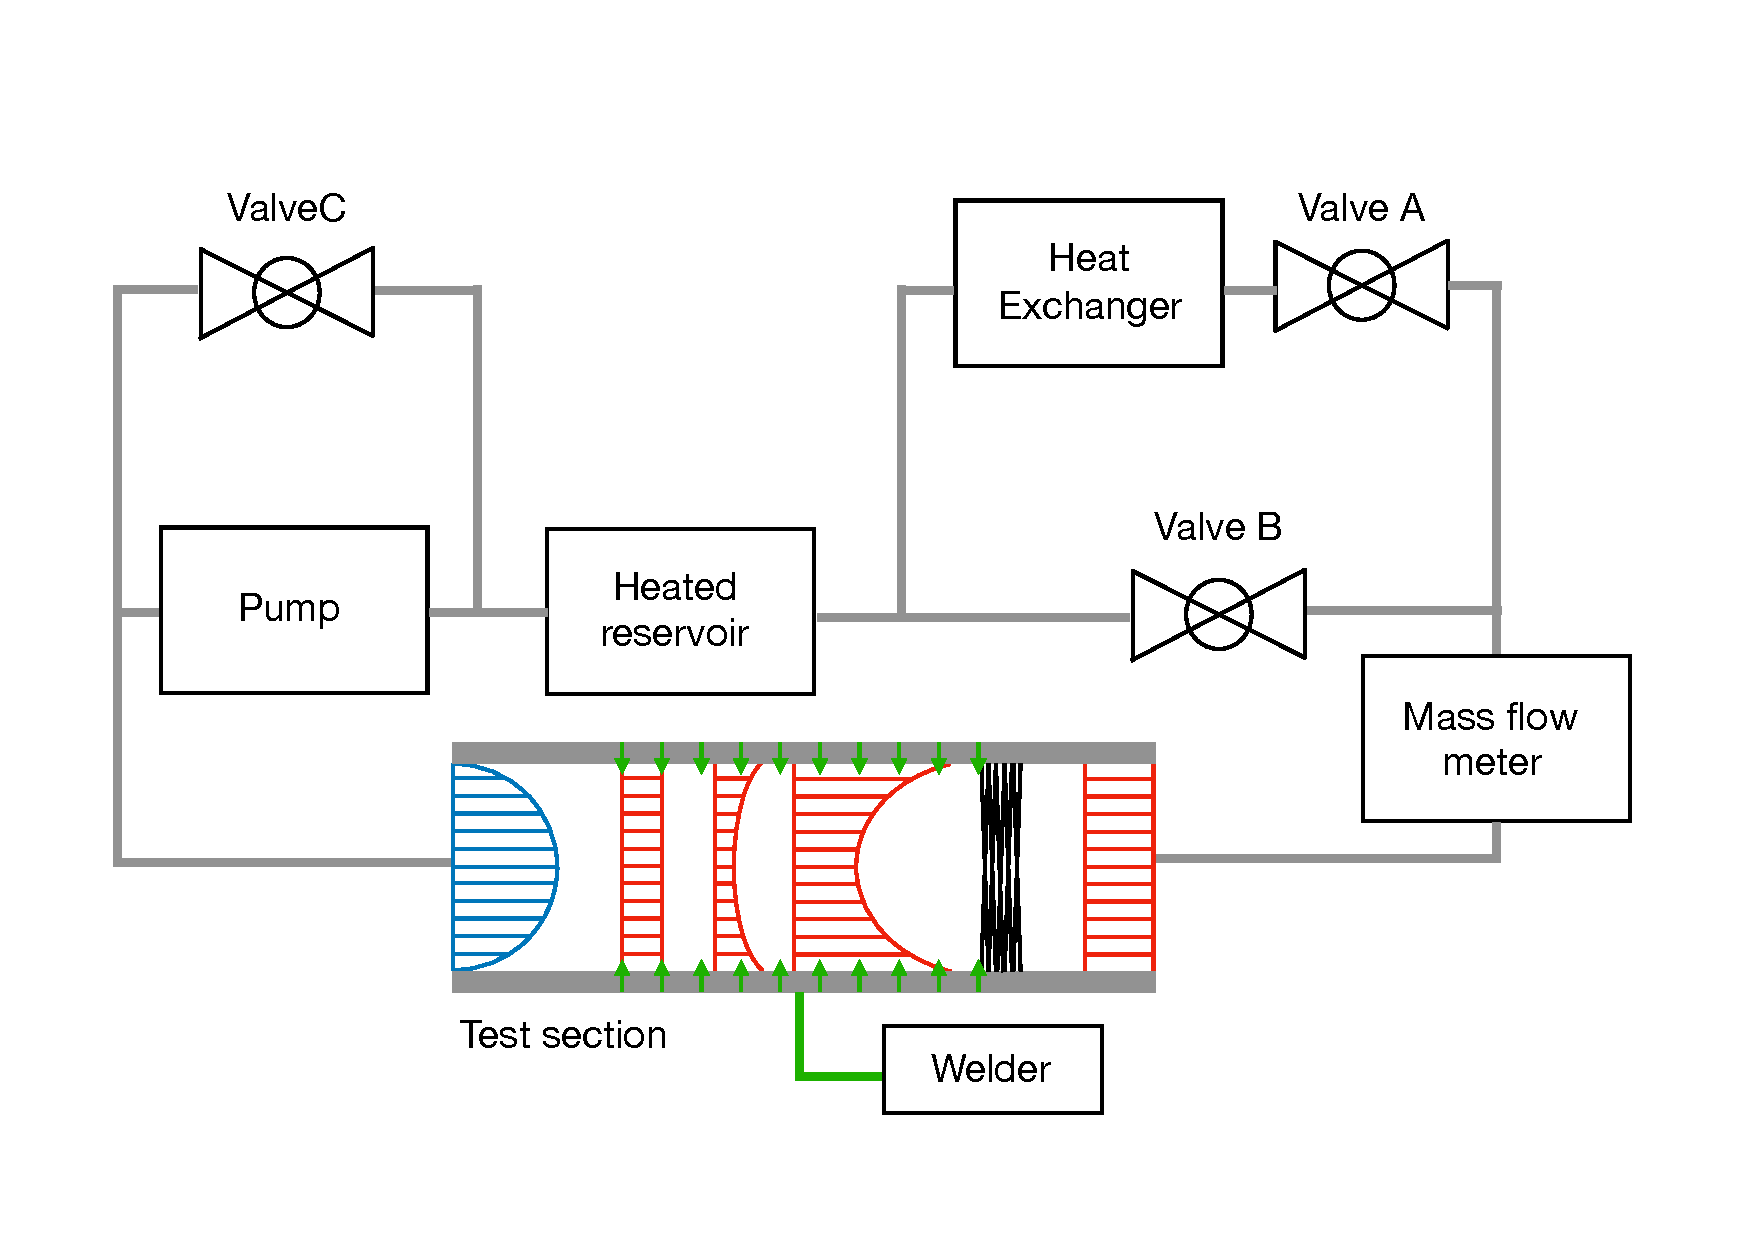
\includegraphics[width=1\linewidth]{fig/loop.pdf}
		\vspace{-3zh}
		\caption{Process flow diagram of the test facilities including test section.}
		\label{loop}
	\end{center}
	\vspace{0zh}
\end{figure}


\section{Test section}

\subsection{Thermal and velocity boundary layer}
Figure. \ref{testsection} shows the velocity and thermal boundary layer of developments vary with the horizontal axis in the test section.
%thermal boundary layer of WHAT???
The velocity and thermal profiles are shown in blue and red color, respectively.
The test section is made of stainless steel (1.4301) with an inner diameter $d_{i}=12[mm]$ and outer diameter $d_{o}=15[mm]$.
Highly accurate resistance thermall probes (PT-100) are used to find out the inlet and outlet bulk temperatures ($T_{in}$, $T_{out}$and wall temperature ($T_{w}$).
Moreover, thermocouples (Type-K) are used to measure temperature gradients in the flow direction.

The test section consists of entrance, heated and thermal equalized parts.
\begin{enumerate}
  \item Entrance part\\
  The first part of the test section is a $1.2\ [m]$ length entrance part, which is sufficiently long to ensure producing dynamically developed flow condition at the exist.
  The bulk temperature $T_{in}$ at this section was measured by PT-100.
  \item Heated part\\
  The second part of the test section is a $2.0\ [m]$ length heated part, which is sufficiently long to ensure producing thermal fully developed flow condition at the exist.
  The tube wall were heated electrically by the welder which provides high current and low voltages to keep the uniform heat flux condition in a inner pipe flow.
  Convective heat transfer is independent of the horizontal axis in fully developed flow and constant heat flux condition.
  The wall temperature $(T_{w})$ at the end of this section were measured by PT-100.
  \item Thermal equalized part\\
  The third part of the test section is the thermall equalized part, which includes a Static mixture.
  The static mixture forms turbulent and vortex.
  Then, the thermal gradients of fluids become averaged, and bull temperature $T_{out}$ is measured.
\end{enumerate}

\begin{figure}[ht]
	\vspace{0zh}
	\begin{center}
		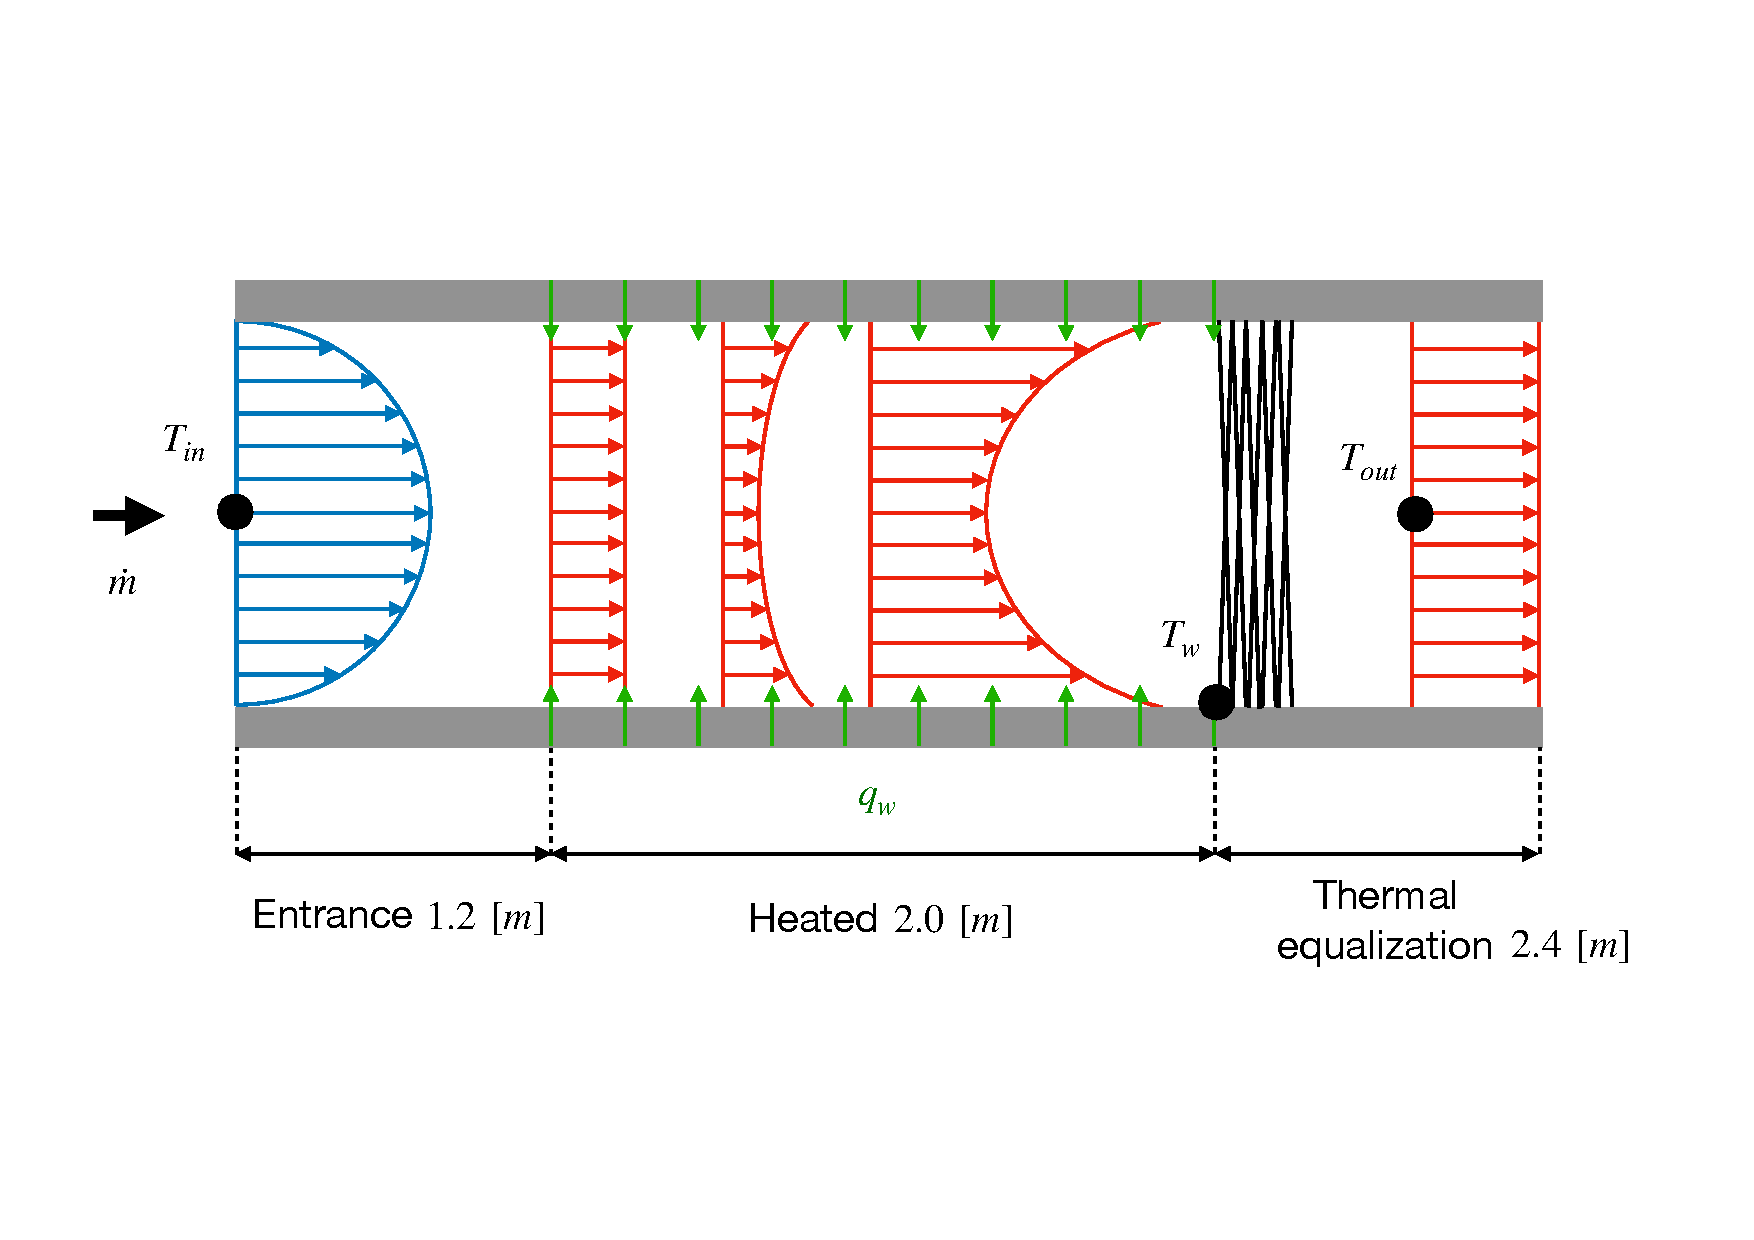
\includegraphics[width=1\linewidth]{fig/testsection.pdf}
		\vspace{-3zh}
		\caption{test section}
		\label{testsection}
	\end{center}
	\vspace{0zh}
\end{figure}

\subsection{Length-to-diameter ratio}
%Ref. Experiments in Pipe Flows at Transitional and Very High Reynolds Numbers p25-
The length-to-diameter ratio is an important parameter to achieve the fully developed turbulent condition in the test section.
The entrance section has an inner diameter of $d_{i}=12mm$, and the length of $L=1.2m$ which length-to-diameter ratio is $L/d_{i}=100$.
Patel et.al.\cite{Zanoun2009} showed suitable the length-to-diameter ratio for fully developed turbulent flows.
According to their study, they found that the minimum developing length of $L/d_{i}=70d_{i}$.
Therefore, the length-to-diameter ratio of the entrance section in this experimental is long enough to ensure the fully developed turbulent flow state.

\section{Conductive heat transfer equation at the pipe wall}
\section{Evaluation procedure}

\clearpage
\section{Uncertainty Analysis of Measurement}
Uncertainty of measurement comprises many components such as bias or systematic error and random error in measuring dimension.
The measured value for dimension is the sum of true value, bias or systematic error and random error as shown in equation \ref{uncertainty_components}.
\begin{equation}
    x = x_{true}+x_{bias}+x_{random}
    \label{uncertainty_components}
\end{equation}
The bias or systematic error may be evaluated from statical distribution and can be characterized by experimental standard deviation.
The uncertainty of measurement was discussed by using ``Guide to the Expression of Uncertainty in Measurement'' \cite{jcgm2008}.

As shown in Chapter ?? in section ??, Reynolds number $Re$, skin friction coefficient $C_{f}$ and Nusselt number $Nu$ was calcurated from following equations (\ref{re_detail})(\ref{cf})(\ref{nu}).
\begin{equation}
    Re = \frac{UL}{\nu} = \frac{4\rho \dot{m}}{\mu \pi d_{i}}
    \label{re_detail}
\end{equation}
\begin{equation}
    C_{f} = \frac{\tau_{w}}{\rho_{b}\frac{U_{b}^{2}}{2}}, \ \tau_{w}=\frac{\Delta P}{\Delta z}\frac{d_{i}}{4}, \ U_{b}=\frac{4\dot{m}}{\rho_{b}\pi d_{i}^{2}}
    \label{cf_detail}
\end{equation}
\begin{equation}
    C_{f} = \frac{\Delta p}{\Delta z} \frac{d_{i}^{5}\pi^{2}\rho_{b}}{32\dot{m}^{2}}
    \label{cf}
\end{equation}
\begin{equation}
   Nu = \frac{\alpha d_{i}}{\lambda} = \frac{q_{w}d_{i}}{\lambda \left( T_{w}-T_{out} \right)}, \ q_{w}=\frac{\dot{m}C_{p} \left( T_{out}-T_{in} \right)}{d_{i}\pi L_{heated}}
   \label{nu_detail}
\end{equation}
\begin{equation}
   Nu = \frac{\dot{m}C_{p,b} \left( T_{out} - T_{in} \right) }{\lambda_{b} \left( T_{w} - T_{out} \right) \pi L_{heated}}
   \label{nu}
\end{equation}
Each parameters effect measurement uncertainty in each sensitivity in sensors.
The right choice of measurement sensors enable us to reduce measurement uncertainty.
However, there is a limitation in reality.
Cramer-Rao lower bound (CRLB) theory indicates the smallest uncertainty limit of estimating variance of deterministic process.
The maximum possible error in equations (\ref{re_detail})(\ref{cf})(\ref{nu}) can be estimated from measurement data.
The uncertainty of skin friction coefficient, $C_{f}$ is calcurated by equation (\ref{delta_cf}).
\begin{equation}
   \Delta C_{f} = \sqrt{\sum \left( \frac{\partial C_{f}}{\partial X_{i}}\Delta X_{i} \right)^{2}}
   \label{delta_cf}
\end{equation}
The uncertainty of skin friction coefficient, $Nu$ is calcurated by equation (\ref{delta_nu}).
\begin{equation}
   \Delta Nu = \sqrt{\sum \left( \frac{\partial Nu}{\partial X_{i}}\Delta X_{i} \right)^{2}}
   \label{delta_nu}
\end{equation}
Here, $\frac{\partial C_{f}}{\partial X_{i}}$ and $\frac{\partial Nu}{\partial X_{i}}$ represents uncertainty elements and assumed to be statistically independent.
In addition, $\Delta X_{i}$ represents absolute error of each sensors.
The resulting total measurement uncertaity in skin friction coefficient is shown in equation (\ref{delta_cf})
\begin{align}
    \Delta C_{f} & = \sqrt{\left(\frac{\partial C_{f}}{\partial \Delta p}\Delta \left( \Delta p \right) \right)^{2} + \left(\frac{\partial C_{f}}{\partial \rho_{out}}\Delta \rho_{out} \right)^{2} + \left(\frac{\partial C_{f}}{\partial \dot{m}}\Delta \dot{m} \right)^{2}}\\
    & = C_{f} \cdot \sqrt{\left( \frac{\Delta \left(\Delta p \right)}{\Delta p}\right)^{2} + \left(\frac{\Delta \rho_{out}}{\rho_{out}}\right)^{2} + \left( 2 \frac{\Delta \dot{m}}{\dot{m}}\right)^{2}}
    \label{delta_cf}
\end{align}

The resulting total measurement uncertaity in Nusselt number is shown in equation (\ref{delta_nu})

\begin{align}
    \Delta Nu & =
    \sqrt{
        \begin{aligned}
        \left(\frac{\partial Nu}{\partial \dot{m}}\Delta \dot{m}\right)^{2} + & \left(\frac{\partial Nu}{\partial c_{p,out}}\Delta c_{p,out}\right)^{2} + \left(\frac{\partial Nu}{\partial \lambda_{out}}\Delta \lambda_{out}\right)^{2} +\\
        & \left(\frac{\partial Nu}{\partial T_{in}}\Delta T_{in}\right)^{2}
        + \left(\frac{\partial Nu}{\partial T_{out}}\Delta T_{out}\right)^{2}
        + \left(\frac{\partial Nu}{\partial T_{w}}\Delta T_{w}\right)^{2}
        \end{aligned}
    }\\
    & = Nu \cdot \sqrt{
        \begin{aligned}
        \left(\frac{\Delta \dot{m}}{\dot{m}}\right)^{2}
        + & \left(\frac{\Delta c_{p,out}}{c_{p,out}}\right)^{2}
        + \left(\frac{\Delta \lambda_{out}}{\lambda_{out}}\right)^{2}+\\
        & \left(\frac{\Delta T}{T_{in} - T_{out}}\right)^{2}
        + \left(\frac{\Delta T}{T_{out} - T_{w}}\right)^{2}
        + \left(\frac{\Delta T\left( T_{in} - T_{w}\right)}{\left( T_{in} - T_{out}\right)\left( T_{out}-T_{w} \right)} \right)^{2}
        \end{aligned}
        }
\end{align}


Table (\ref{absolute_error}) shows absolute error for each sensors.
As shown in material properties, density, heat capasity and heat conductivity are temperature dependence.
Therefore, those absolute error influenced by the sensitivity of the temperature sensor, PT100.
\begin{table}[h]
\centering
\caption{Absolute error of contribution factor of the Reynolds number, skin friction coefficient and Nusselt number.}
\vspace{1zh}
\label{absolute_error}
\begin{tabular}{llll} \toprule%\boldmath
{Contribution} & {Symbol}          & {Absolute error}   & {Unit}\\ \midrule
Mass flow rate & $\Delta \dot{m}$  & $0.20E-3\dot{m}$   & $kg\cdot s^{-1}$\\
Pressure       & $\Delta(\Delta p)$& $0.35E-3\Delta p$  & $Pa$\\
Temperature    & $\Delta T$        & 0.040              & $K$\\
Density        & $\Delta \rho_{out}$& $0.26E-1$         & $kg\cdot m^{-3}$\\
Thermal conductivity & $\lambda_{out}$& $2.4E-5$        & $W\cdot m^{-1}\cdot K^{-1}$\\
Heat capasity  & $\Delta c_{p,out}$& 0.18               & $J\cdot kg^{-1}\cdot K^{-1}$\\
\bottomrule
\end{tabular}
\end{table}

\clearpage
\subsection{Case study}
In this section, the author showed evaluation procedure to calcurate measurement uncertainty for Reynolds number, skin friction coefficient and Nusselt number, respectively.
For this case study, Table (\ref{case_study}) shows one of the measurement data in this study.

\begin{table}[h]
\centering
\caption{Concrete exaples for evaluation procedure of uncertainty analysis. Comprehensive measurement result of the data is shown in Chapter??.}
\vspace{1zh}
\label{case_study}
\begin{tabular}{lllllllllllll} \toprule%\boldmath
{Case} & {$Pr_{w}$} & {$Re$}  & {$C_{f}$} & {$Nu$} & {$\dot{m}$} & {$\Delta p$} & {$T_{w}$} & {$T_{in}$} & {$T_{out}$} & {$\rho_{out}$} & {$\lambda_{out}$} & $c_{p,out}$\\ \midrule
A & 10.0 & 3747 & 0.0103 & 39  & 0.044 & 254  & 71.2 & 65.2 & 67.6 & 1041 & 0.42 & 3.55\\
B & 10.0 & 18626& 0.0068 & 152 & 0.212 & 3816 & 71.3 & 69.5 &70.1&
1042 & 0.42 & 3.56\\
\bottomrule
\end{tabular}
\end{table}

Measurement uncertainty for Reynolds number was shown in equation ---


Measurement uncertainty for skin friction coefficient was shown in equation (\ref{delta_cf}).
By substituting absolute error shown in table (\ref{absolute_error}) into the equation (\ref{delta_cf}), which yeilds
\begin{equation}
   \Delta C_{f} = C_{f} \cdot \sqrt{\left( \frac{0.35E-3\Delta p}{\Delta p}\right)^{2} + \left(\frac{0.26E-1}{\rho_{out}}\right)^{2} + \left( 2\ \frac{0.20E-3\dot{m}}{\dot{m}}\right)^{2}}
   \label{case_study_cf1}
\end{equation}
Then, by substituting measurement data shown in table (\ref{case_study})into equation (\ref{delta_cf}), measurement uncertainty for skin friction ocefficient is calcurated.
\begin{align}
    \Delta C_{f} & = 0.0103 \cdot \sqrt{\left( \frac{0.35E-3\cdot 253.8}{253.8}\right)^{2} + \left(\frac{0.26E-1}{1041}\right)^{2} +   \left( 2\ \frac{0.20E-3\cdot 0.044}{0.044}\right)^{2}}\\
    &= 0.0103 \cdot \sqrt{ \left( 0.00035 \right)^{2} + \left( 0.0004 \right)^{2} + \left( 0.000025 \right)^{2} }\\
    &= 5.5E-6
   \label{case_study_cf2}
\end{align}

Measurement uncertainty for Nusselt number was shown in equation (\ref{delta_nu}).
By substituting absolute error shown in table (\ref{absolute_error}) into the equation (\ref{delta_nu}), which yeilds
\begin{align}
    \Delta Nu & = Nu\cdot
    \sqrt{
    \begin{aligned}
        & \left(\frac{0.20E-3\dot{m}}{\dot{m}}\right)^{2}
        + \left(\frac{0.18}{c_{p,out}}\right)^{2}
        + \left(\frac{2.4E-5}{\lambda_{out}}\right)^{2}+\\
        & \left(\frac{0.0040}{T_{in} - T_{out}}\right)^{2}
        + \left(\frac{0.0040}{T_{out} - T_{w}}\right)^{2}
        + \left(\frac{0.0040\cdot \left( T_{in} - T_{w}\right)}{\left( T_{in} - T_{out}\right)\left( T_{out}-T_{w} \right)} \right)^{2}
    \end{aligned}
          }\\
    & = 38.7\cdot
    \sqrt{
    \begin{aligned}
        & \left(\frac{0.20E-3\cdot 0.044}{0.044}\right)^{2}
        + \left(\frac{0.18}{3.55E+3}\right)^{2}
        + \left(\frac{2.4E-5}{0.420}\right)^{2}+\\
        & \left(\frac{0.0040}{65.2 - 67.6}\right)^{2}
        + \left(\frac{0.0040}{67.6 - 71.2}\right)^{2}
        + \left(\frac{0.0040\cdot \left(65.2 - 71.2\right)}{\left(65.2 - 67.6\right)\left(67.6 - 71.2\right)}\right)^{2}
    \end{aligned}
         }\\
    & = 38.7\cdot
    \sqrt{
    \begin{aligned}
        \left(0.20E-3\right)^{2} +
        & \left(0.51E-4\right)^{2}
        + \left(0.57E-4\right)^{2} +\\
        & \left(0.16E-2\right)^{2}
        + \left(0.10E-2\right)^{2}
        + \left(0.27E-2\right)^{2}
    \end{aligned}
         }\\
    & = 0721
\end{align}








\chapter{Experiments}
\section{Parameter valiation during experiment}
\clearpage

\section{Validation of experimental result for $Pr_{w}=10$}
\subsection{Skin friction coefficient for $Pr_{w}=10$}
In previous studies friction coefficient have been established by many researches.
Since the friction coefficient is independet to temperature and exactly known, validity of the experimental data were checked.
Figure (\ref{pr10_recf}) shows skin frictin coefficient $C_{f}$ and bulk Reynolds number $Re_{b}$ for $Pr_{w} = 10$ compared with DNS and emperical correlations for laminar and turbulent as shown in Equations (\ref{cf_laminar})(\ref{cf_turbulent}).

\begin{figure}[ht]
	\vspace{0zh}
	\begin{center}
		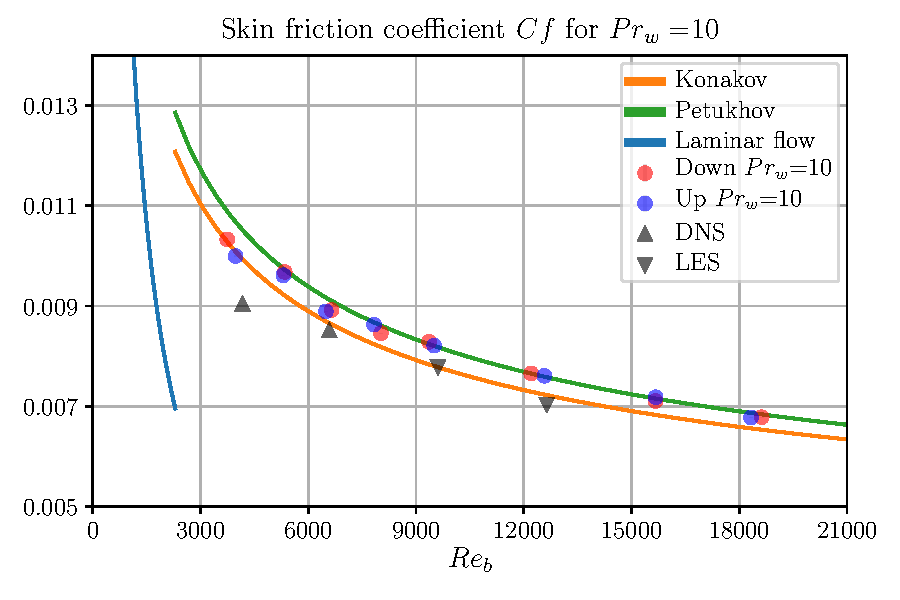
\includegraphics[width=0.9\linewidth]{fig/pr10_recf.pdf}
		\vspace{-1zh}
		\caption{The comparison between skin frictin coefficient $C_{f}$ and bulk Reynolds number $Re_{b}$ for $Pr_{w} = 10$}
		\label{pr10_recf}
	\end{center}
	\vspace{0zh}
\end{figure}


Every measurement was performed twice to check the reproducibility of the results.
The measurement points were taken from lower to higher Reynolds number (red points) and higher to lower Reynolds number (blue points).
The reproducibility decreases for lower Reynolds numbers, as can be seen in Figure  (\ref{pr10_recf}).

Each measurement points were averaged value in 420 samples as show in Cahpter??.
There was a scattering observed especialy for Low Reynolds number.
Detailed discussion is show in Chapter??.

\clearpage
\subsection{Heat transfer coefficient for $Pr_{w}=10$}
Figure (\ref{pr10_renu}) shows heat transfer coefficient $Nu$ and bulk Reynolds number $Re_{b}$ for $Pr_{w} = 10$ compared with DNS and Gnielinski correlations for laminar (\ref{Nu_laminar}), transitional (\ref{Nu_transitional}) and turbulent (\ref{Nu_turbulent}).

\begin{figure}[ht]
	\vspace{0zh}
	\begin{center}
		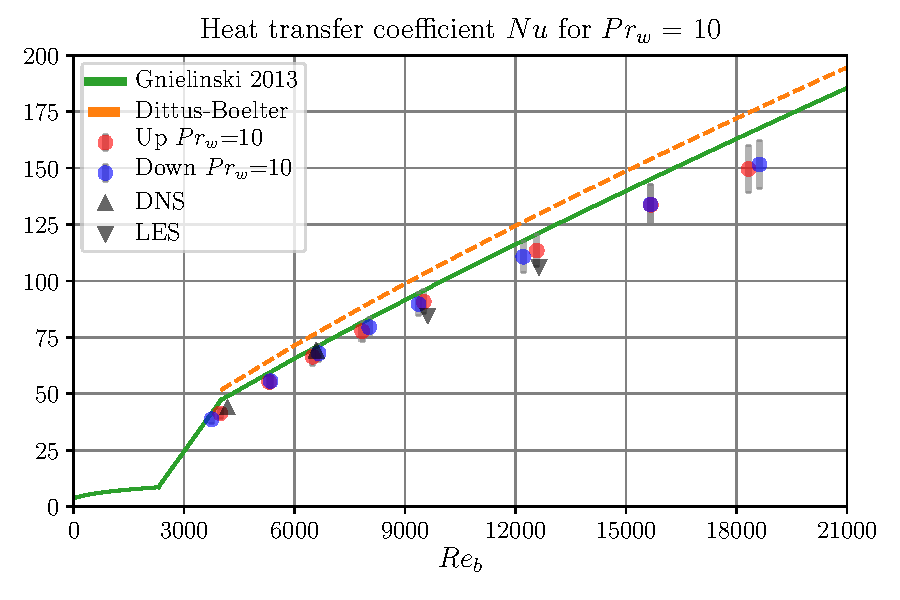
\includegraphics[width=0.9\linewidth]{fig/pr10_renu.pdf}
		\vspace{-1zh}
		\caption{The comparison between heat transfer coefficient $Nu$ and bulk Reynolds number $Re_{b}$ for $Pr_{w} = 10$}
		\label{pr10_renu}
	\end{center}
	\vspace{0zh}
\end{figure}

As mensioned before, every measurement was performed twice to check the reproducibility of the results.
A quantitative analysis to determine measurement uncertainties was applied, based on the maximum deviation of the measured and calculated values.
Using this approach, the gray error bar in the figures shows measurement uncertainties.
The eveluation procedure is shown in Chapter??.

As can be seen in Figure (\ref{pr10_renu}), it is obvious that the measurement on Nusselt number for $3747<Re_{b}<9508$ are very well fitted by the Gnielinski correlation(\ref{Nu_turbulent}).
However, for $Re_{b}>12207$, the measurement are under estimated and out of the measurement uncertainty.

Table (\ref{pr10_updown}) shows summary of the experimental parameters for $Pr_{w}=10$ and performance of the skin friction coefficient $C_{f}$ and Nusselt number $Nu$.

\begin{table}[h]
\centering
\caption{Summary of the experimental parameters for $Pr_{w}=10$ and performance of the skin friction coefficient\ $C_{f}$ and Nusselt number\ $Nu$}
\vspace{1zh}
\label{pr10_updown}
\begin{tabular}{lSrrSlSSSSS}
\toprule%\boldmath
{Type} & {{$Pr_{w}$}} & {$Re_{b}$} & {$C_{f}$} & {$Nu$} & {$T_{in}$} & {$T_{out}$} &  {$T_{w}$} & {$\Delta T$}  & {$\Delta \mu/ \mu_{b}$} & {$q_{w, hc}$} \\
{}&{-}&{-}&{$\times10^{-3}$}&{-}&{$^\circ C$}&{$^\circ C$}&{$^\circ C$}&{$^\circ C$}&{\%}&{$kWm^{-2}$}\\\midrule %& {$q_{el}\ [kW/m^{2}]$}
Up & 10.0 & 3981  & 9.99  & 41.3 & 65.4 & 67.8 & 71.4 & 3.6  & 6.2  & 5.3\\
     & 9.9  & 5309  & 9.61  & 55.2 & 66.4 & 68.5 & 71.6 & 3.1  & 5.3  & 6.0\\
     & 10.0 & 6493  & 8.89  & 66.4 & 67.0 & 68.7 & 71.3 & 2.5  & 4.4  & 5.9\\
     & 10.0 & 7833  & 8.63  & 77.8 & 67.7 & 69.1 & 71.4 & 2.2  & 3.9  & 6.1\\
     & 10.0 & 9508  & 8.21  & 90.8 & 68.1 & 69.4 & 71.3 & 1.9  & 3.3  & 6.1\\
     & 10.0 & 12575 & 7.61  & 113.4& 68.9 & 69.8 & 71.4 & 1.6  & 2.8  & 6.4\\
     & 10.0 & 15674 & 7.18  & 113.7& 69.5 & 70.2 & 71.5 & 1.3  & 2.2  & 6.1\\
     & 10.0 & 18328 & 6.78  & 149.6& 69.6 & 70.2 & 71.4 & 1.2  & 2.0  & 6.1\\
\midrule
Down & 10.0 & 3747  & 10.33 & 38.7 & 65.2 & 67.6 & 71.2 & 3.6  & 6.2  & 4.8\\
     & 10.0 & 5348  & 9.68  & 55.6 & 66.4 & 68.3 & 71.2 & 2.9  & 4.9  & 5.6\\
     & 10.0 & 6654  & 8.92  & 67.9 & 67.0 & 68.7 & 71.2 & 2.5  & 4.3  & 5.9\\
     & 10.0 & 8026  & 8.46  & 79.5 & 67.7 & 69.2 & 71.4 & 2.2  & 3.8  & 6.2\\
     & 10.0 & 9365  & 8.28  & 89.7 & 68.0 & 69.2 & 71.2 & 1.9  & 3.4  & 6.1\\
     & 10.0 & 12207 & 7.66  & 110.7& 68.9 & 69.9 & 71.5 & 1.6  & 2.8  & 6.3\\
     & 10.0 & 15668 & 7.10  & 113.8& 69.3 & 70.1 & 71.4 & 1.3  & 2.3  & 6.2\\
     & 10.0 & 18626 & 6.78  & 151.6& 69.5 & 70.1 & 71.3 & 1.2  & 2.0  & 6.2\\
\bottomrule
\end{tabular}
\end{table}

%\% of the data were whithin \pm 10\%


\clearpage
\subsection{Skin friction coefficient vary with heat flux for $Pr_{w}=10$}
Data obtained in previous studies \cite{Everts2018} using water as test liquid indicated that providing higher heat flux resulted in lower skin friction coefficient.
According to DNS result with using water-glycole, the same trend were observed.
In this study, the dependency of wall heat flux were obtained for both skin friction coefficient and heat transfer coefficient.
Figure \ref{pr10_recf_heatflux} shows the results obtained with variety of wall heat flux compared with emperical correlations Petukhov and Konakov \cite{Petukhov1970} and DNS results.

\begin{figure}[ht]
	\vspace{0zh}
	\begin{center}
		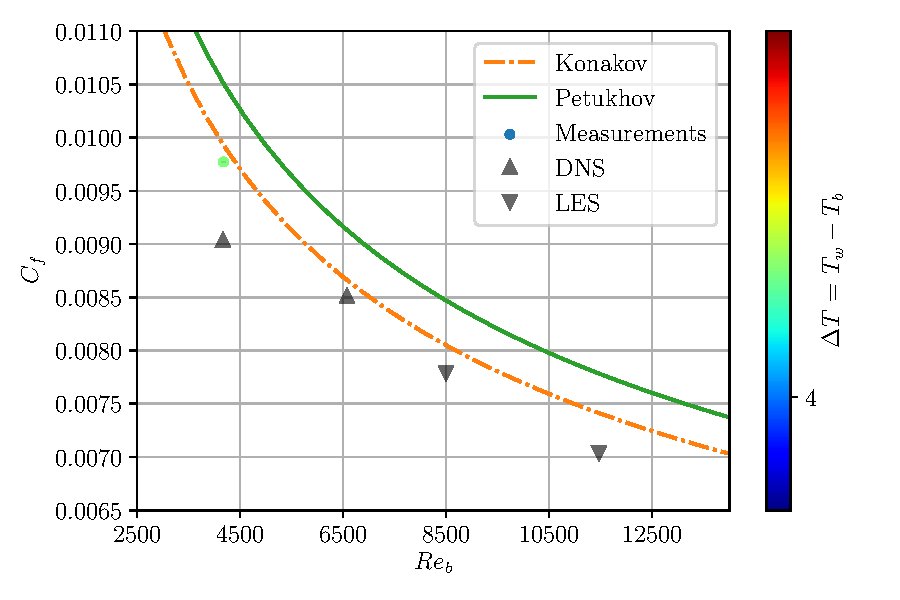
\includegraphics[width=1\linewidth]{fig/pr10heatflux_recfdt.pdf}
		\vspace{-3zh}
		\caption{The comparison between skin frictin coefficient $C_{f}$ and bulk Reynolds number $Re_{b}$ for $Pr_{w} = 10$ vary with temperature defference $\Delta T$ between a pipe wall $T_{w}$ and the bulk $T_{b}$.}
		\label{pr10_recf_heatflux}
	\end{center}
	\vspace{0zh}
\end{figure}

As can be seen,

\clearpage
\subsection{Heat transfer coefficient vary with heat flux for $Pr_{w}=10$}
In general, it is apparent that heat transfer coefficient dcrease for higher heat flux.

\begin{figure}[ht]
	\vspace{0zh}
	\begin{center}
		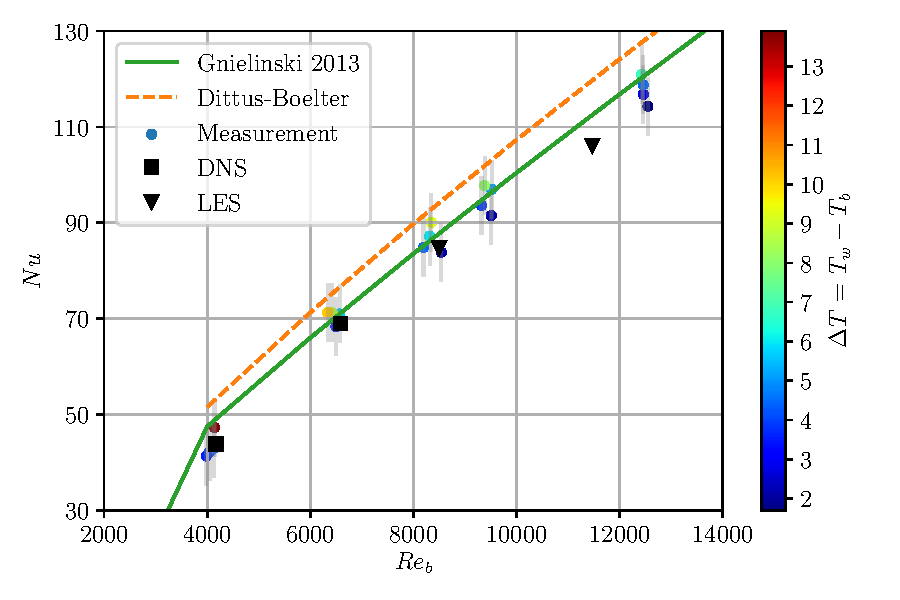
\includegraphics[width=1\linewidth]{fig/pr10heatflux_renudt.pdf}
		\vspace{-3zh}
		\caption{The comparison between heat transfer coefficient $Nu$ and bulk Reynolds number $Re_{b}$ for $Pr_{w} = 10$ vary with temperature defference $\Delta T$ between a pipe wall $T_{w}$ and the bulk $T_{b}$.}
		\label{pr10_renu_heatflux}
	\end{center}
	\vspace{0zh}
\end{figure}

As can be seen,

Table (\ref{pr10_heatflux}) summarises the range for Reynolds number and wall heat flux for $Pr_{w}=10$ realized during experiments.

\begin{table}[h]
\centering
\caption{Summary of the experimental parameters for $Pr_{w}=10$ and performance of the skin friction coefficient\ $C_{f}$, Nusselt number\ $Nu$ and temperature defference\ $\Delta T=T_{w}-T_{b}$.}
\vspace{1zh}
\label{pr10_heatflux}
\begin{tabular}{SrrSlSSSSS} \toprule%\boldmath
{{$Pr_{w}$}} & {$Re_{b}$} & {$C_{f}$} & {$Nu$} & {$T_{in}$} & {$T_{out}$} &  {$T_{w}$} & {$\Delta T$}  & {$\Delta \mu/ \mu_{b}$*} & {$q_{w}$**} \\
{-}&{-}&{$\times10^{-3}$}&{-}&{$^\circ C$}&{$^\circ C$}&{$^\circ C$}&{$^\circ C$}&{\%}&{$kWm^{-2}$}\\\midrule %& {$q_{el}\ [kW/m^{2}]$}
10.0 & 4176  & 9.77  & 43.5 & 64.4 & 67.2 & 71.4 & 4.2  & 7  & 6.5  \\%& 8.1
9.9  & 4029  & 10.20 & 44.1 & 58.9 & 63.7 & 71.6 & 7.9  & 14 & 12.3 \\%& 14.8
10.0 & 4098  & 9.68  & 45.6 & 56.5 & 62.2 & 71.3 & 9.1  & 16 & 14.6 \\%& 16.8
10.0 & 3948  & 9.77  & 45.1 & 49.9 & 57.9 & 71.5 & 13.5 & 23 & 21.5 \\%& 25.2
\midrule
10.0 & 6496  & 8.97  & 68.3 & 65.3 & 67.8 & 71.5 & 3.7  & 6  & 8.9  \\%& 11.1
10.0 & 6569  & 8.69  & 71.0 & 61.9 & 65.6 & 71.3 & 5.7  & 10 & 14.1 \\%& 16.8
9.9  & 6423  & 8.79  & 71.2 & 57.2 & 62.8 & 71.5 & 8.8  & 15 & 22.0 \\%& 25.7
10.0 & 6337  & 9.20  & 71.3 & 54.8 & 61.1 & 71.4 & 10.2 & 17 & 25.6 \\%& 30.0
\midrule
10.0 & 8540  & 8.36  & 83.9 & 67.8 & 69.2 & 71.5 & 2.2  & 4  & 6.6  \\%& 8.7
10.0 & 8194  & 8.43  & 84.9 & 64.0 & 66.9 & 71.4 & 4.5  & 8  & 13.4 \\%& 16.3
10.0 & 8315  & 8.47  & 87.2 & 61.6 & 65.4 & 71.4 & 6.0  & 10 & 18.5 \\%& 21.9
10.0 & 8347  & 8.48  & 90.1 & 56.5 & 62.1 & 71.4 & 9.3  & 16 & 29.6 \\%& 34.1
\midrule
9.9  & 9508  & 8.09  & 91.5 & 68.2 & 69.5 & 71.5 & 2.1 & 4  & 6.6  \\%& 8.8
10.0 & 9320  & 8.19  & 93.6 & 65.1 & 67.5 & 71.4 & 3.9 & 7  & 12.8 \\%& 15.6
10.0 & 9518  & 8.15  & 97.0 & 62.9 & 66.1 & 71.3 & 5.2 & 9  & 17.8 \\%& 21.2
9.9  & 9380  & 8.18  & 97.8 & 58.8 & 63.6 & 71.7 & 8.1 & 14 & 27.8 \\%& 32.4
\midrule
10.0 & 11628 & 7.48  & 107.4 & 68.8 & 69.8 & 71.5 & 1.7 & 3  & 6.5  \\%& 8.8
9.8  & 11445 & 7.67  & 108.7 & 67.7 & 69.4 & 72.1 & 2.8 & 5  & 10.7 \\%& 13.3
10.0 & 11213 & 7.74  & 110.5 & 63.4 & 66.4 & 71.5 & 5.0 & 9  & 19.6 \\%& 23.1
9.9  & 11373 & 7.84  & 113.4 & 60.4 & 64.5 & 71.7 & 7.2 & 12 & 28.7 \\%&33.4
\midrule
10.0 & 12548 & 7.38  & 114.3 & 68.7 & 69.7 & 71.4 & 1.7 & 3  & 6.7  \\%& 8.9
10.0 & 12458 & 7.46  & 116.8 & 66.9 & 68.6 & 71.4 & 2.8 & 5  & 11.7 \\%& 14.6
9.9  & 12457 & 7.61  & 118.8 & 64.5 & 67.1 & 71.6 & 4.5 & 8  & 19.0 \\%& 22.6
9.9  & 12427 & 7.59  & 121.0 & 60.8 & 64.7 & 71.6 & 6.8 & 12 & 29.1 \\%& 33.6
\bottomrule
\end{tabular}
\end{table}


\begin{table}[h]
\centering
\caption{Direct Numerical Simuration\ (DNS) and Large Eggy Simuration\ (LES) for $Pr_{w} = 10$ vary with heat flux $q_{w}=20\ [kW/m^{2}]$ and $q_{w}=?\ [kW/m^{2}]$}
\vspace{1zh}
\label{simuration}
\begin{tabular}{lllrrrllllrl} \toprule
{Type} & {$Pr_{w}$} & {$Re_{\tau}$}& {$Re_{b}$} & {$C_{f}$} & {$Nu$} & {$T_{w}\ [^\circ C]$} & {$T_{b}\ [^\circ C]$}  & {$\Delta T\ [^\circ C]$}  & {$q_{w}\ [kW/m^{2}]$} \\ \midrule
DNS & 10.0 & 360 & 4165  & 0.00904 & 43.8  & 71.2 & 58.5 & 13.1 & 20.0  \\
DNS & 10.0 & 360 & 4165  & ?       & ?     & 71.2 & ?    & ?    & 40.0  \\ \midrule
DNS & 10.0 & 500 & 6587  & 0.00851 & 69.0  & 71.2 & 63.3 & 8.3  & 20.0 \\
DNS & 10.0 & 500 & 6587  & ?       & ?     & 71.2 & ?    & ?    & 40.0 \\ \midrule
LES & 10.0 & 600 & 8498  & 0.00779 & 84.8  & 71.2 & 64.8 & 6.8  & 20.0 \\ \midrule
LES & 10.0 & 750 & 11465 & 0.00704 & 106.1 & 71.2 & 66.2 & 5.4  & 20.0 \\ \bottomrule
\end{tabular}
\end{table}

\clearpage
\section{Validation of experimental result for $Pr_{w}=7, 13$}
\subsection{Skin friction coefficient for $Pr_{w}=7, 13$}

\begin{figure}[ht]
	\vspace{0zh}
	\begin{center}
		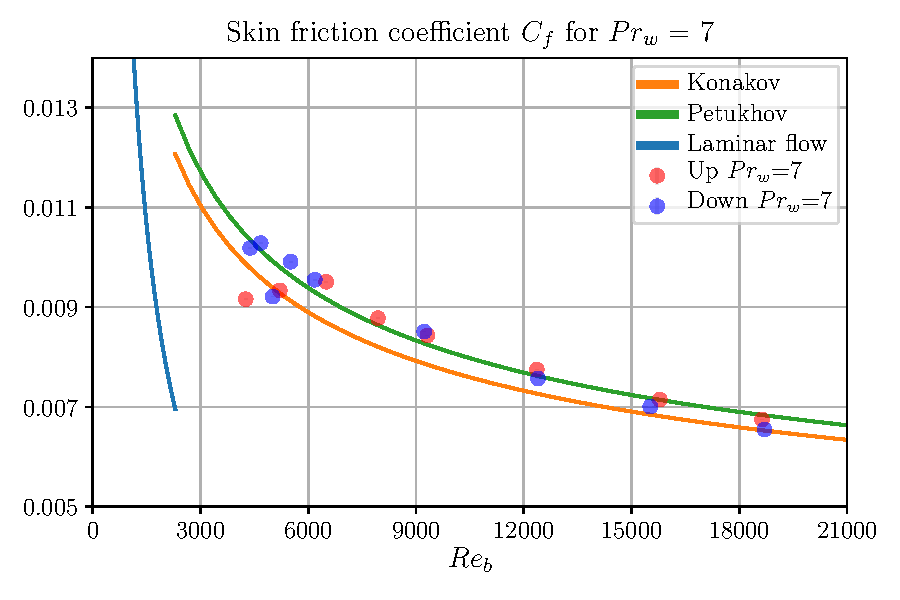
\includegraphics[width=0.9\linewidth]{fig/pr7_recf.pdf}
		\vspace{-1zh}
		\caption{The comparison between skin frictin coefficient $C_{f}$ and bulk Reynolds number $Re_{b}$ for $Pr_{w} = 7$}
		\label{pr7_recf}
	\end{center}
	\vspace{0zh}
\end{figure}

\begin{figure}[ht]
	\vspace{0zh}
	\begin{center}
		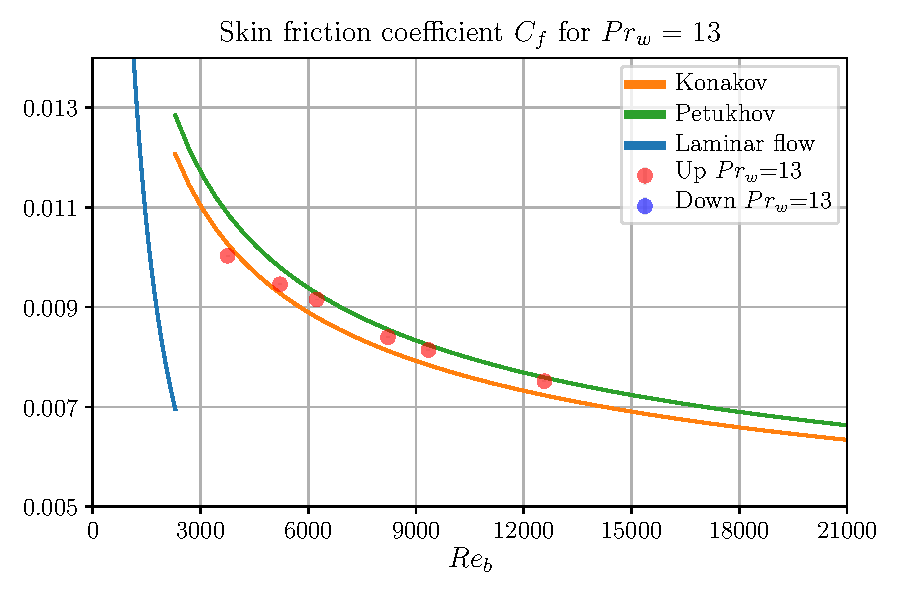
\includegraphics[width=0.9\linewidth]{fig/pr13_recf.pdf}
		\vspace{-1zh}
		\caption{The comparison between skin frictin coefficient $C_{f}$ and bulk Reynolds number $Re_{b}$ for $Pr_{w} = 13$}
		\label{pr13_recf}
	\end{center}
	\vspace{0zh}
\end{figure}


\clearpage
\subsection{Heat transfer coefficient for $Pr_{w}=7, 13$}

\begin{figure}[ht]
	\vspace{0zh}
	\begin{center}
		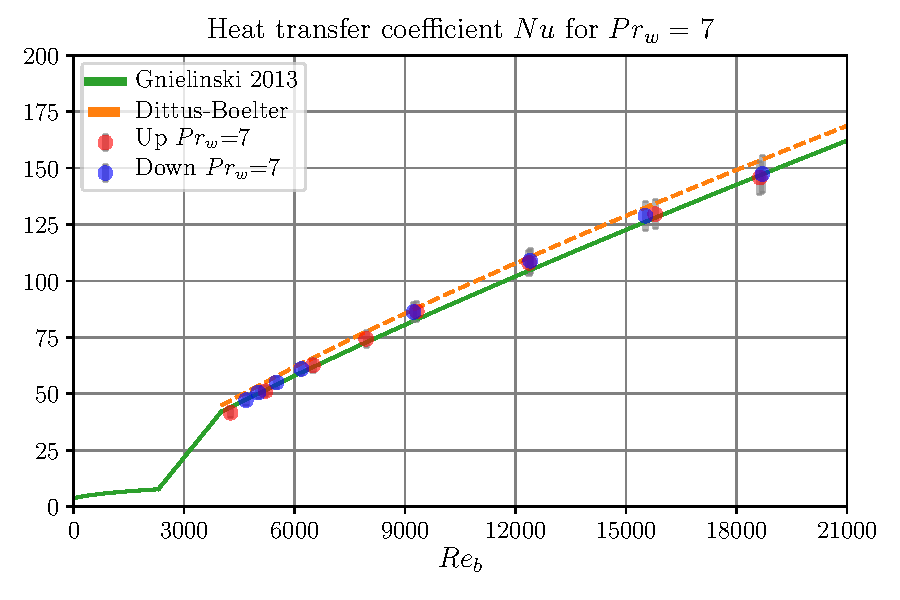
\includegraphics[width=0.9\linewidth]{fig/pr7_renu.pdf}
		\vspace{-1zh}
		\caption{The comparison between heat transfer coefficient $Nu$ and bulk Reynolds number $Re_{b}$ for $Pr_{w} = 7$}
		\label{pr7_renu}
	\end{center}
	\vspace{0zh}
\end{figure}

\begin{figure}[ht]
	\vspace{0zh}
	\begin{center}
		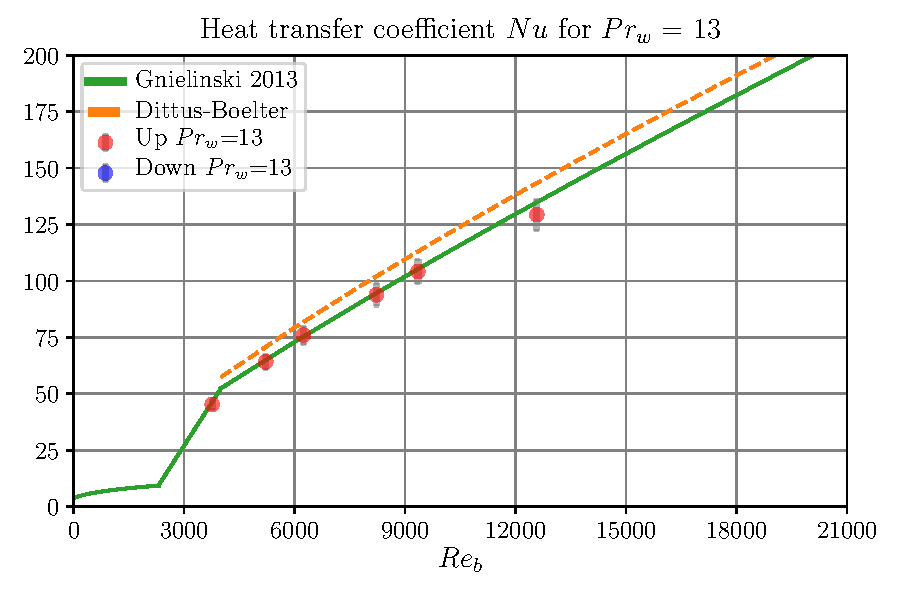
\includegraphics[width=0.9\linewidth]{fig/pr13_renu.pdf}
		\vspace{-1zh}
		\caption{The comparison between heat transfer coefficient $Nu$ and bulk Reynolds number $Re_{b}$ for $Pr_{w} = 13$}
		\label{pr13_renu}
	\end{center}
	\vspace{0zh}
\end{figure}

\clearpage
\begin{table}[h]
\centering
\caption{Summary of the experimental parameters for $Pr_{w}=7$ and performance of the skin friction coefficient\ $C_{f}$ and Nusselt number\ $Nu$}
\vspace{1zh}
\label{pr07_updown}
\begin{tabular}{lSrrSlSSSSS}
\toprule%\boldmath
{Type} & {{$Pr_{w}$}} & {$Re_{b}$} & {$C_{f}$} & {$Nu$} & {$T_{in}$} & {$T_{out}$} &  {$T_{w}$} & {$\Delta T$}  & {$\Delta \mu/ \mu_{b}$*} & {$q_{w}$**} \\
{}&{-}&{-}&{$\times10^{-3}$}&{-}&{$^\circ C$}&{$^\circ C$}&{$^\circ C$}&{$^\circ C$}&{\%}&{$kWm^{-2}$}\\\midrule %& {$q_{el}\ [kW/m^{2}]$}
Up   & 6.9  & 4261  & 9.16  & 41.6 & 82.7 & 88.8 & 95.7 & 6.9  & 8.6  & 10.0\\
     & 7.0  & 5211  & 9.34  & 51.2 & 84.9 & 89.8 & 95.3 & 5.4  & 6.8  & 10.1\\
     & 7.0  & 6500  & 9.51  & 62.6 & 86.8 & 90.8 & 95.3 & 4.5  & 5.6  & 10.3\\
     & 7.0  & 7943  & 8.78  & 74.3 & 88.5 & 91.7 & 95.4 & 3.7  & 4.6  & 10.0\\
     & 7.0  & 9317  & 8.43  & 86.5 & 84.4 & 89.3 & 95.2 & 5.9  & 7.4  & 18.6\\
     & 7.0  & 12366 & 7.75  & 108.0& 85.3 & 89.9 & 95.6 & 5.6  & 7.1  & 22.2\\
     & 7.0  & 15790 & 7.14  & 129.6& 86.2 & 90.1 & 95.4 & 5.3  & 6.6  & 25.1\\
     & 7.0  & 18634 & 6.75  & 145.7& 86.6 & 90.2 & 95.4 & 5.2  & 6.5  & 27.6\\
\midrule
Down & 7.0  & 4287  & 9.90  & 42.9 & 77.0 & 85.5 & 95.5 & 10.0 & 12.5 & 15.6\\
     & 7.0  & 4385  & 10.19 & 44.1 & 77.2 & 85.5 & 95.1 & 9.6  & 12.1 & 15.5\\
     & 7.0  & 4679  & 10.29 & 47.2 & 78.1 & 86.0 & 95.1 & 9.1  & 11.4 & 15.6\\
     & 7.0  & 5012  & 9.21  & 50.5 & 78.8 & 86.3 & 95.0 & 8.7  & 11.0 & 16.0\\
     & 6.9  & 5513  & 9.91  & 55.0 & 79.3 & 86.9 & 95.7 & 8.8  & 11.0 & 17.6\\
     & 6.9  & 6183  & 9.55  & 61.0 & 80.6 & 87.6 & 95.7 & 8.1  & 10.1 & 18.0\\
     & 7.0  & 9231  & 8.51  & 86.2 & 83.2 & 88.6 & 95.3 & 6.6  & 8.3  & 20.8\\
     & 7.0  & 12399 & 7.57  & 108.9& 84.3 & 89.2 & 95.5 & 6.3  & 7.9  & 25.0\\
     & 6.9  & 15523 & 7.00  & 128.8& 85.1 & 89.6 & 95.7 & 6.1  & 7.6  & 28.7\\
     & 7.0  & 18700 & 6.55  & 147.3& 91.6 & 93.2 & 95.3 & 2.1  & 2.7  & 11.5\\
\bottomrule
\end{tabular}\\
\text{* A viscosity ratio of pipe wall and center.$\Delta \mu = \mu_{b}-\mu_{w}$.}\\
\text{** Heat flux calcurated from heat capacity equation which directly connected with temperature difference between inlet $T_{in}$ and outlet $T_{out}$.}
\end{table}


\begin{table}[h]
\centering
\caption{Summary of the experimental parameters for $Pr_{w}=13$ and performance of the skin friction coefficient\ $C_{f}$ and Nusselt number\ $Nu$}
\vspace{1zh}
\label{pr13_updown}
\begin{tabular}{lSrrSlSSSSS}
\toprule%\boldmath
{Type} & {{$Pr_{w}$}} & {$Re_{b}$} & {$C_{f}$} & {$Nu$} & {$T_{in}$} & {$T_{out}$} &  {$T_{w}$} & {$\Delta T$}  & {$\Delta \mu/ \mu_{b}$*} & {$q_{w}$**} \\
{}&{-}&{-}&{$\times10^{-3}$}&{-}&{$^\circ C$}&{$^\circ C$}&{$^\circ C$}&{$^\circ C$}&{\%}&{$kWm^{-2}$}\\\midrule %& {$q_{el}\ [kW/m^{2}]$}
Up   & 13.0  & 3760  & 10.03  & 45.3 & 46.0 & 50.0 & 57.7 & 7.8  & 16.2  & 12.1\\
     & 13.0  & 5217  & 9.46   & 64.1 & 45.7 & 49.9 & 57.9 & 8.0  & 16.6  & 17.6\\
     & 12.9  & 6239  & 9.16   & 76.0 & 45.6 & 49.9 & 58.1 & 8.2  & 17.0  & 21.5\\
     & 12.9  & 8221  & 8.40   & 93.8 & 49.4 & 52.3 & 57.9 & 5.6  & 11.8  & 18.3\\
     & 12.9  & 9348  & 8.14   & 104.2& 49.3 & 52.3 & 58.2 & 5.9  & 12.3  & 21.2\\
     & 12.9  & 12577 & 7.52   & 129.4& 50.9 & 53.1 & 57.9 & 4.8  & 10.0  & 21.4\\
     &&&&&&&&&&\\
     &&&&&&&&&&\\
\midrule
Down &&&&&&&&&&\\
\bottomrule
\end{tabular}
\end{table}






\clearpage
\subsection{Skin friction coefficient vary with heat flux for $Pr_{w}=7, 13$}
\begin{figure}[ht]
	\vspace{0zh}
	\begin{center}
		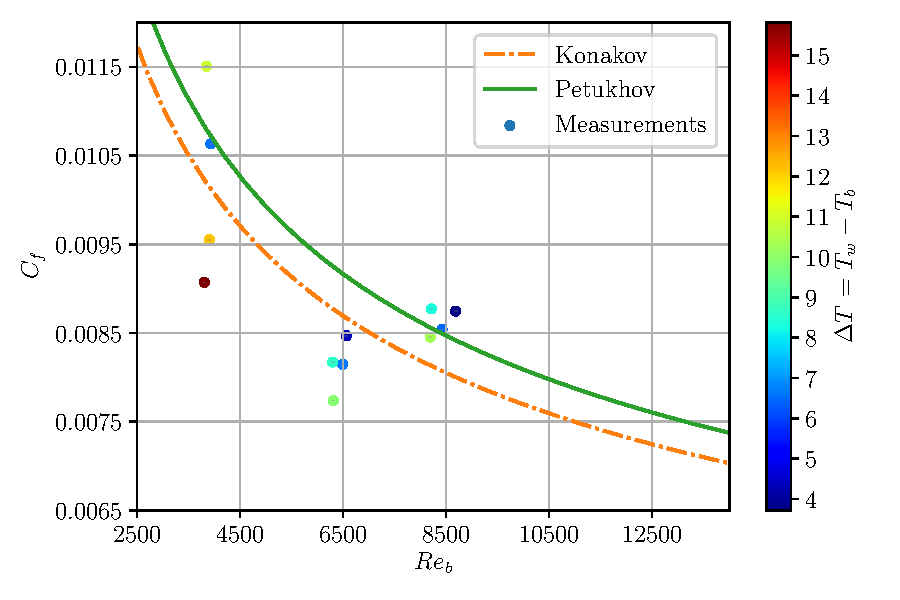
\includegraphics[width=1\linewidth]{fig/pr7heatflux_recfdt.pdf}
		\vspace{-3zh}
		\caption{The comparison between skin frictin coefficient $C_{f}$ and bulk Reynolds number $Re_{b}$ for $Pr_{w} = 7$ vary with temperature defference $\Delta T$ between a pipe wall $T_{w}$ and the bulk $T_{b}$.}
		\label{pr7_recf_heatflux}
	\end{center}
	\vspace{0zh}
\end{figure}

\begin{figure}[ht]
	\vspace{0zh}
	\begin{center}
		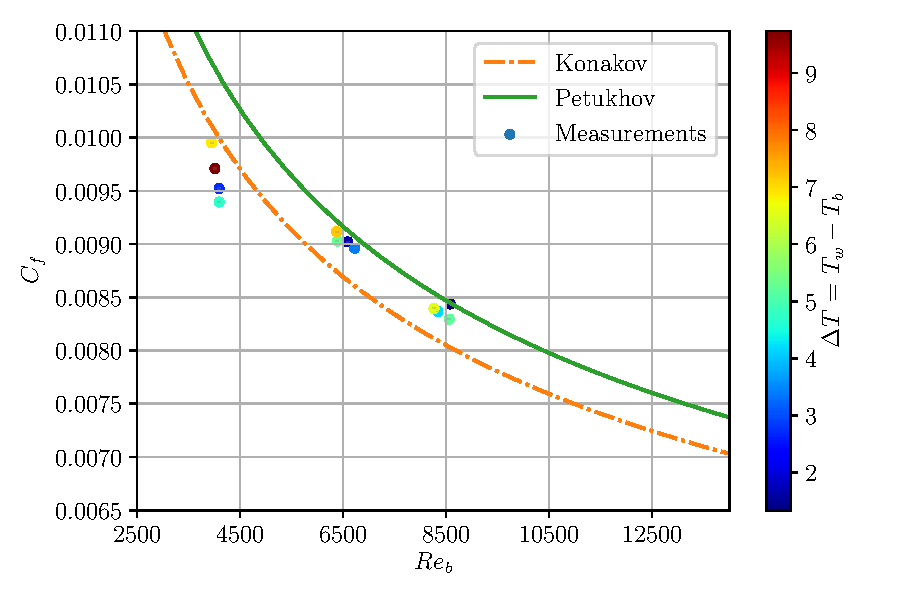
\includegraphics[width=1\linewidth]{fig/pr13heatflux_recfdt.pdf}
		\vspace{-3zh}
		\caption{The comparison between skin frictin coefficient $C_{f}$ and bulk Reynolds number $Re_{b}$ for $Pr_{w} = 13$ vary with temperature defference $\Delta T$ between a pipe wall $T_{w}$ and the bulk $T_{b}$.}
		\label{pr13_recf_heatflux}
	\end{center}
	\vspace{0zh}
\end{figure}


\clearpage
\subsection{Heat transfer coefficient vary with heat flux for $Pr_{w}=7, 13$}
\begin{figure}[ht]
	\vspace{0zh}
	\begin{center}
		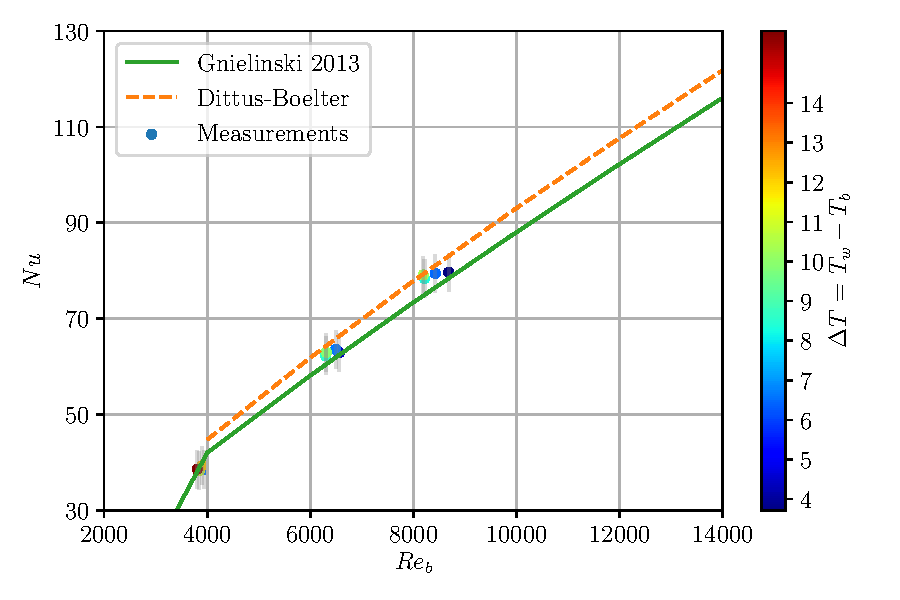
\includegraphics[width=1\linewidth]{fig/pr7heatflux_renudt.pdf}
		\vspace{-3zh}
		\caption{The comparison between heat transfer coefficient $Nu$ and bulk Reynolds number $Re_{b}$ for $Pr_{w} = 7$ vary with temperature defference $\Delta T$ between a pipe wall $T_{w}$ and the bulk $T_{b}$.}
		\label{pr7_renu_heatflux}
	\end{center}
	\vspace{0zh}
\end{figure}

\begin{figure}[ht]
	\vspace{0zh}
	\begin{center}
		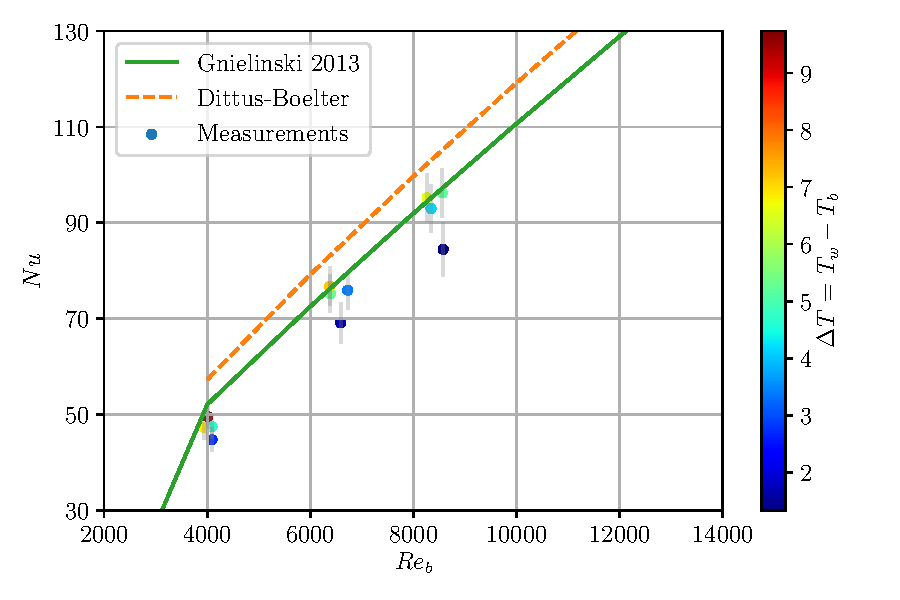
\includegraphics[width=1\linewidth]{fig/pr13heatflux_renudt.pdf}
		\vspace{-3zh}
		\caption{The comparison between heat transfer coefficient $Nu$ and bulk Reynolds number $Re_{b}$ for $Pr_{w} = 13$ vary with temperature defference $\Delta T$ between a pipe wall $T_{w}$ and the bulk $T_{b}$.}
		\label{pr13_renu_heatflux}
	\end{center}
	\vspace{0zh}
\end{figure}

\begin{table}[h]
\centering
\caption{Summary of the experimental parameters for $Pr_{w}=7$ and performance of the skin friction coefficient\ $C_{f}$, Nusselt number\ $Nu$ and temperature defference\ $\Delta T=T_{w}-T_{b}$.}
\vspace{1zh}
\label{pr7_heatflux}
\begin{tabular}{SrrSlSSSSS} \toprule%\boldmath
{{$Pr_{w}$}} & {$Re_{b}$} & {$C_{f}$} & {$Nu$} & {$T_{in}$} & {$T_{out}$} &  {$T_{w}$} & {$\Delta T$}  & {$\Delta \mu/ \mu_{b}$*} & {$q_{w}$**} \\
{-}&{-}&{$\times10^{-3}$}&{-}&{$^\circ C$}&{$^\circ C$}&{$^\circ C$}&{$^\circ C$}&{\%}&{$kWm^{-2}$}\\\midrule %& {$q_{el}\ [kW/m^{2}]$}
7    & 4176  & 9.77  & 43.5 & 64.4 & 67.2 & 71.4 & 4.2  & 7  & 6.5  \\
\midrule
7    & 6496  & 8.97  & 68.3 & 65.3 & 67.8 & 71.5 & 3.7  & 6  & 8.9  \\
\midrule
7    & 8540  & 8.36  & 83.9 & 67.8 & 69.2 & 71.5 & 2.2  & 4  & 6.6  \\
\midrule
7    & 9508  & 8.09  & 91.5 & 68.2 & 69.5 & 71.5 & 2.1 & 4  & 6.6  \\
\bottomrule
\end{tabular}
\end{table}

\begin{table}[h]
\centering
\caption{Summary of the experimental parameters for $Pr_{w}=13$ and performance of the skin friction coefficient\ $C_{f}$, Nusselt number\ $Nu$ and temperature defference\ $\Delta T=T_{w}-T_{b}$.}
\vspace{1zh}
\label{pr13_heatflux}
\begin{tabular}{SrrSlSSSSS} \toprule%\boldmath
{{$Pr_{w}$}} & {$Re_{b}$} & {$C_{f}$} & {$Nu$} & {$T_{in}$} & {$T_{out}$} &  {$T_{w}$} & {$\Delta T$}  & {$\Delta \mu/ \mu_{b}$*} & {$q_{w}$**} \\
{-}&{-}&{$\times10^{-3}$}&{-}&{$^\circ C$}&{$^\circ C$}&{$^\circ C$}&{$^\circ C$}&{\%}&{$kWm^{-2}$}\\\midrule %& {$q_{el}\ [kW/m^{2}]$}
13  & 4176  & 9.77  & 43.5 & 64.4 & 67.2 & 71.4 & 4.2  & 7  & 6.5  \\
\midrule
13  & 6496  & 8.97  & 68.3 & 65.3 & 67.8 & 71.5 & 3.7  & 6  & 8.9  \\
\midrule
13  & 8540  & 8.36  & 83.9 & 67.8 & 69.2 & 71.5 & 2.2  & 4  & 6.6  \\
\midrule
13  & 9508  & 8.09  & 91.5 & 68.2 & 69.5 & 71.5 & 2.1 & 4  & 6.6  \\
\bottomrule
\end{tabular}
\end{table}


\clearpage
\section{Discussion}
\subsection{Reproducibility}
\subsection{Secoundary flow}
\subsection{Electric shield}
%\subsection{Influence of heat flux}


\clearpage
\subsection{Trendency of scattering}
%In this study, the author found that for lower Reynodls number,
%As lower Reynolds number, higher scattering for skinf friction coefficient.
Figure shows prresure and velocity oscilatin dependence of time axis.
Each red crossing points shows measurement samples of each time and the samples were taken every one second.
---------------\\
As shown in figures, both pressure and velocity has fraqutuation dependent of time.
In order to investigate the relationship between skin friction coefficient, prresure and velocit, cross correlation function were calcurated.
Table show cross correlation for each factors.
\begin{table}

\end{table}

--------------\\
Table shows standard deviation of each parameters for $Re_{b}=??$ and $Re_{b}=??$.
As shown in the table, the scattering of those parametes are independ to the Reynolds number.
However, the scattering for skin friction coefficient decrease for higher Reynolds number.
As shown in Chapter??, skin friction coefficient is deriverded following eqaution. (\ref{cf})
\begin{equation}
    C_{f} = \frac{\Delta p}{\Delta z} \frac{d_{i}^{5}\pi^{2}\rho_{b}}{32\dot{m}^{2}}
    \label{cf}
\end{equation}
The skin fricition coefficiet is proposal to prresure differene $\Delta p$ and ?? to mass flow rate $\dot{m}$ which is directly connected to valocity$U$.
For higher Reynolds number which means higer velosity, skin friction coefficient decrease ??? to the power of mass flow rate.
Therefore, the effect of pressure scatering seems to dcrease because of high velocity term.\\
\subsection{Electric field from a welder}
Skin friction coefficient without heating from the welder could not observe any scattering.
The welder achieve high current, and we assumed the scatering come from electric field from the welder.
Then, a cable of pressure sensor was surrounded to protect from the eleceric field.\\
Figure shows standard deviation with and without electrical shield.
It is ovbsiou that the electical shield achieve to decrease the pressure noise from the welder.
\begin{figure}[t]
    \begin{minipage}{0.5\hsize}
        \begin{center}
            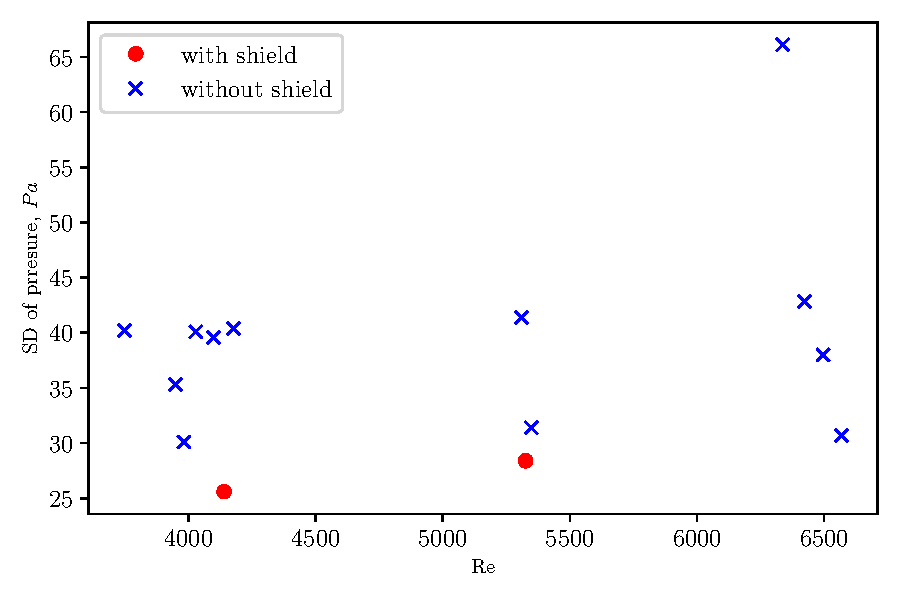
\includegraphics[width=1\linewidth]{fig/SD_shield4prresure.pdf}
        \end{center}
        \caption{一つめの図}
        \label{fig:one}
    \end{minipage}
    \begin{minipage}{0.5\hsize}
        \begin{center}
            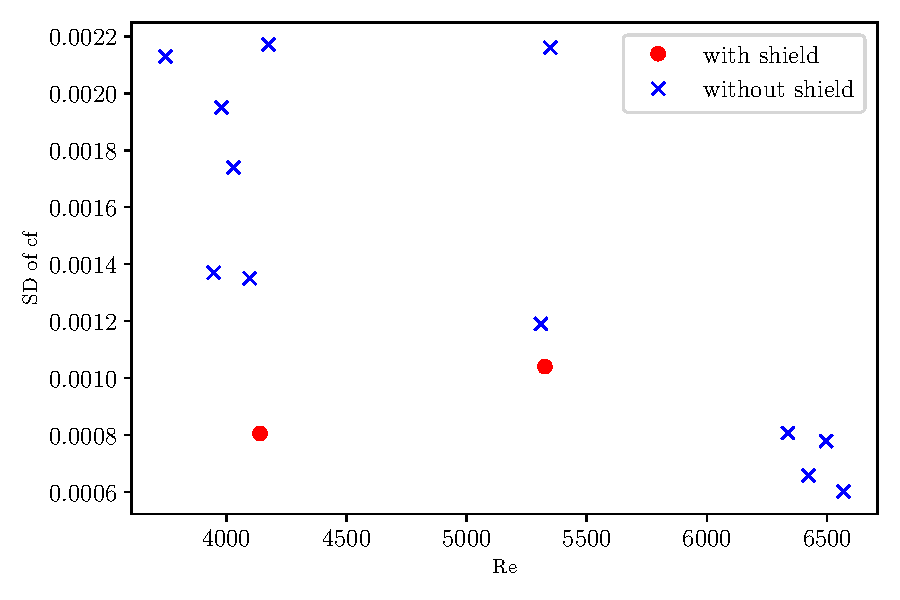
\includegraphics[width=1\linewidth]{fig/SD_shield4cf.pdf}
        \end{center}
        \caption{二つめの図}
        \label{fig:two}
    \end{minipage}
\end{figure}
Comparing Fig () and (), it is obvious that a significant improvement was obtained in the majority of cases.
As you can see from the figures, ???$\%$ of the scattering is reduced.


\subsection{Probability density function}


\subsection{Comparison with Bertsche}
\subsection{Comparison with DNS and LES}
\subsection{Effect of the presure popower}
\subsection{Effect of material properties}

\chapter{Conclusion}


\appendix
%% !TEX root = ../thesis-sample.tex
\appendix
\doublespacing
\chapter{Material properties}
A 50/50vol\% mixture of water and glycole which is a typical liquid coolant in automotive applications were used as a operating fluid.

\chapter{Post processing}
\lipsum[24]


%http://lightology.hatenablog.com/entry/2018/02/12/221721
\bibliographystyle{amsplain}
\bibliography{/Users/Shared/TeXLive/texmf/bibtex/bib/local/graz.bib}
%\bibitem{Frank}Frank P.Incropera et al., ``Fundamentals of Heat and Mass Transfer'', (Wiley, 2006)

\end{document}
